%%%%%%%%%%%%%%%%%%%%%%%%%%%%%%%%%%%%%%%%%%%%%%%%%%
%% Bachelor's & Master's Thesis Template        %%
%% Copyleft by Dawid Weiss & Marta Szachniuk    %%
%% Faculty of Computing and Telecommunication   %%
%% Poznan University of Technology, 2020        %%
%%%%%%%%%%%%%%%%%%%%%%%%%%%%%%%%%%%%%%%%%%%%%%%%%%


\documentclass[english,master,a4paper,oneside]{ppfcmthesis}


\usepackage[utf8]{inputenc}
\usepackage[T1]{fontenc}

%--------------------------------------
% Title page
%--------------------------------------

\author{%
   Dominik Maćkowiak \album{151915}}
\authortitle{}

\title{Interpretable methods for data-to-text generation}

\ppsupervisor{Mateusz Lango, PhD}

\ppyear{2026}


\begin{document}

% Front matter starts here
\frontmatter\pagestyle{empty}%
\maketitle\cleardoublepage%

%--------------------------------------
% Diploma thesis card placeholder
%--------------------------------------

\thispagestyle{empty}\vspace*{\fill}%
\begin{center}Here the diploma thesis card will be placed;\\ insert the original for the PP archive copy, a photocopy for the remaining copies.\end{center}%
\vfill\cleardoublepage%

%--------------------------------------
% Abstract
%--------------------------------------

\thispagestyle{empty}
\vspace*{2cm}
\begin{center}
\Large\textbf{Abstract}
\end{center}
\vspace{1cm}

% Abstract content goes here
\chapter*{Abstract}

This thesis proposes an interpretable method for data-to-text generation from structured data. The generation process is divided into two stages: constructing a meaning representation and performing rule-based surface realization. This enables automatic or human evaluation of text semantics and explicit tracing of the text-generation process, rather than relying on a single, non-interpretable generation step.

Three pipelines for constructing meaning representations as RDF triples using large language models are proposed and evaluated. The Text-First Extraction with Normalization pipeline achieves the strongest reported results, while the remaining methods provide greater control over the predicate set and auditable intermediate artifacts. A domain-specific model is also trained to distill the operation of the complete processing pipelines into a single inference step. Training with QLoRA adapters substantially improves triple extraction over the base model, although performance depends on the domain and evaluation metric.

For surface realization, the thesis proposes using OpenEvolve to construct verbalization rules expressed as executable Python code. The evolutionary process uses LLM-generated code mutations and automatic text-evaluation metrics as objective functions. Experiments conducted on the WebNLG dataset show that optimizing reference-based evaluation metrics and metrics based on the LLM-as-Judge paradigm produces surface realizers with different properties. The evolved programs do not surpass the text quality achieved by a fine-tuned BART model or by zero-shot LLM generation, but they provide transparent and reproducible realization logic that can be inspected and modified without using an LLM at inference time.

The results confirm that explicit intermediate representations and executable generation artifacts are practical tools for interpretable data-to-text generation.


\vfill\cleardoublepage%

%--------------------------------------
% Table of contents
%--------------------------------------

\pagenumbering{Roman}\pagestyle{ppfcmthesis}%
\tableofcontents*
\cleardoublepage

%--------------------------------------
% Chapters
%--------------------------------------

\mainmatter%

\chapter{Introduction}

\section{Motivation}

Data-to-text (D2T) generation concerns the automatic conversion of structured
information into natural-language text. It is useful whenever information stored
as records, tables, databases, time series, or knowledge graphs must be converted
in a linguistic form, which is more suitable for a human reader, a conversational
interface, or another language-based system. D2T systems must therefore solve
two related problems: they must select and organize the information that should
be communicated, and then express that information in text that is fluent,
coherent, and faithful to its source
\cite{gatt2018survey,osuji2024systematic}.

Recent neural and large language model based systems have substantially improved
the fluency and flexibility of generated text. However, fluent text does not
necessarily preserve the content of the input. A system may omit a fact,
introduce an unsupported statement, select different facts on different
executions in a way that changes their apparent
meaning. Additionally, a direct neural generator, these intermediate choices are not usually
represented as explicit objects that a developer can inspect, modify, or compare
with the source. This makes it difficult to identify whether an error resulted
from content selection, content ordering, aggregation, lexicalization, or surface
realization.
\cite{wiseman-etal-2017-challenges,dusek-kasner-2020-evaluating,
dhingra-etal-2019-handling}.

Before neural generation became dominant, D2T systems were commonly built using
manually authored rules and templates. A rule-based system specifies conditions
and operations for selecting, ordering, and combining facts, while a template
provides a sentence pattern into which values can be inserted. Such systems are
easy to inspect and can provide strong control over which source facts are
realized. Their limitation is not that rules are inherently expensive, but that
the engineering effort grows as the task becomes more varied. New predicates,
combinations of facts, aggregation patterns, domains, and linguistic constructions
may each require additional design, testing, and maintenance
\cite{reiter1997building,gatt2018survey}.

This challenge is especially visible for complex structured data. A time series,
for example, may require decisions about temporal ordering, aggregation,
extremes, trends, and the level of detail appropriate for the output. These
decisions are not caused by the presence of time alone; they arise because the
system must handle many possible structures and realizations. Neural systems
reduce some of this manual engineering and offer greater linguistic variety, but
their learned generation behavior is harder to inspect.

One way to make this trade-off more manageable is to separate meaning
representation from surface realization. A meaning representation is an
intermediate, structured description of the content to be communicated. It is
independent of the exact wording of the final text and can be expressed using,
for example, logical forms, semantic frames, text plans, or graphs. An explicit
meaning representation makes the selected content available for inspection before
it is verbalized. The resulting decomposition can be summarized as
\begin{equation}
    d \longrightarrow T \longrightarrow y,
\end{equation}
where $d$ denotes a structured data instance, $T$ denotes its interpretable meaning
representation, and $y$ denotes the generated text. In this context,
interpretability means that the intermediate meaning representation and the procedure
that produces the text are explicit artifacts that can be inspected.
Meaning representation make the facts being communicated explicit and provide an intermediate
object that can be inspected, normalized, and evaluated independently of the
final wording. Nevertheless, constructing consistent meaning representation from complex data
and producing fluent text from it remains non-trivial tasks.

Existing work has shown that LLMs can be used to construct an interpretable
rule-based meaning representation to text generator.
Lango and Dušek~\cite{lango-dusek-2025-llm} use cooperating LLM agents to design
and refine such a generator (a Python program), from meaning representation, which can be inspected, executed without an LLM at inference time, and corrected by a developer when necessary.

The scope of that approach begins after a meaning representation has already
been provided: it addresses just the surface realization.
A further limitation of a fixed sequence of agent interactions is that it does
not by itself define a systematic criterion for comparing many alternative
generators. Agents can propose and critique changes, but their next
action is primarily guided by the current conversation.

For these reasons, the objective of this thesis is to considers the complete D2T pipeline, from heterogeneous
raw structured instances through an explicit meaning representation to the final
text.
Separating these two stages also
allows errors introduced during meaning-representation construction to be
distinguished from errors introduced during surface realization.
In the first stage an
LLM-based pipeline is used for the meaning-representation construction. A domain-specialized
model is also examined as a way of producing both the meaning representation and a text in a single inference pass.
In the second stage, the surface-realization method used in this thesis places an
LLM inside an evolutionary optimization loop inspired by AlphaEvolve
\cite{novikov2025alphaevolve}, a framework for evolutionary program improvement
using LLM-generated mutations and automatic evaluation.
The advantage of such an approach over the agents is that it evaluates every proposed program using the same
evaluator, retains high-scoring and structurally diverse candidates, and uses
the accumulated results to guide subsequent modifications. This makes it
possible to reject plausible but ineffective changes and to revisit alternative
realization strategies rather than relying on a single refinement trajectory.
Reference-based and semantic metrics are used to evaluate generation quality and faithfulness.
Interpretability is supported by exposing the meaning representation and the human-readable program code.

The work makes the following contributions:
\begin{itemize}
    \item three LLM-based pipeline designs are proposed for constructing meaning representation
    from heterogeneous structured data;
    \item a domain-specialized training procedure that distills the
    conversion process into a large language model;
    \item an evolutionary surface-realization method in which LLM-generated
    program mutations are executed and selected using automatic evaluation;
    \item a systematic empirical evaluation of the proposed methods across
    multiple domains using reference-based, semantic, and LLM-based measures.
\end{itemize}

\section{Thesis structure}

The structure of the thesis is as follows. Chapter~2 introduces the D2T task,
reviews the principal generation approaches, discusses interpretability, and
describes the evaluation methods used in this area. Chapter~3 presents the
meaning-representation construction stage of the proposed pipeline. It describes
how complex structured instances are converted into meaning representation using
LLM-based pipelines and a domain-specialized fine-tuned model.

Chapter~4 presents the surface-realization stage, namely the conversion of
semantic triples into natural-language text. It introduces the AlphaEvolve and
OpenEvolve frameworks and explains how an executable program for verbalizing
triples is selected, mutated, evaluated, and retained during evolution.
Chapter~5 describes the experimental datasets and configurations, reports the
results for meaning-representation construction and surface realization, and
evaluates the complete pipeline. Chapter~6 discusses the results, limitations,
and broader implications of the proposed approach. Finally, Chapter~7
summarizes the thesis and presents its conclusions. The appendices contain the
prompts used by the conversion methods and the initial surface-realization
program.


\chapter{Data-to-Text Generation}

Data-to-text (D2T) generation is a branch of natural language generation in
which a system converts structured input data into natural-language text
\cite{gatt2018survey,osuji2024systematic}. Inputs may be tables, database
records, time series, or graphs. The output should communicate the source
content fluently, coherently, and without unsupported statements. D2T is thus a
mapping from a structured input representation to a linguistic output.

\section{Problem definition}
\label{sec:d2t-problem-definition}

\subsection{Data-to-Text task}

The general aim of D2T generation is to produce a textual description $y$ from
structured input $x$:
\begin{equation}
    G(x) = y,
\end{equation}
where $G$ is a data-to-text generator. 

D2T is distinguished from text-to-text generation by the nature of its source.
In machine translation, summarization, and paraphrasing, the input is already
natural language. In D2T, the generator must determine what the source data
means for the current communicative purpose, organize that content into a
discourse, and realize the resulting plan as sentences. The
required output can range from a short dialogue utterance to a multi-sentence
report or a complete document~\cite{gatt2018survey,osuji2024systematic}.

The generated text is normally expected to satisfy several requirements.
\emph{Faithfulness} concerns whether every expressed statement is supported by
the source; incorrect values and additions are faithfulness errors.
\emph{Adequacy} concerns whether the selected content is appropriate for the
communicative purpose, while \emph{coverage} concerns omissions among facts
that the task requires the text to communicate. The output should also be
grammatical, fluent, coherent, and appropriately organized.

\subsection{RDF and semantic triples}
\label{sec:rdf-semantic-triples}

The Resource Description Framework (RDF) is a graph-based data model for
representing statements about resources~\cite{w3c2014rdf11concepts}. The basic
unit of an RDF statement is a triple consisting of a subject, a predicate, and
an object. The subject identifies the entity being described, the predicate
denotes a relation or property, and the object identifies another entity or
contains a literal value. A compact representation of a statement about a
mobile phone can therefore be written as:
\begin{equation}
    (\texttt{ex:PhoneModel},\ \texttt{ex:hasBatteryCapacity},\ \texttt{"5000 mAh"}).
\end{equation}
Here, \texttt{ex:} is a namespace prefix, \texttt{ex:PhoneModel} is the
subject, \texttt{ex:hasBatteryCapacity} is the predicate, and the string
\texttt{"5000 mAh"} is the object literal. In a complete RDF representation,
resources and predicates are normally identified using globally resolvable
identifiers, while literals may carry datatypes or language tags.

A collection of RDF triples forms a directed, labeled graph: subjects and
resource objects are nodes, and predicates label the edges between them. The
same entity can participate in many relations, and an object can simultaneously
be the subject of other statements. RDF does not itself determine how the facts
should be ordered or aggregated in a text~\cite{w3c2014rdf11concepts}. It can
therefore serve as a \emph{meaning representation}: an explicit,
structured representation of content that has been selected for communication.
It preserves the selected facts
and their relations while leaving wording, sentence structure, and discourse
organization to the \emph{surface realization}: the process of converting the
meaning representation into natural language.

In this thesis, a simplified version of RDF triples are used, which can be written as
\begin{equation}
    T = \{(s_i,p_i,o_i)\}_{i=1}^{n},
\end{equation}
where $s_i$ is a subject, $p_i$ is a predicate, and $o_i$ is an object. From now on in the thesis, the name
\emph{semantic triples}, or just \emph{triples} will be used to refer to this simplified representation. 
It has the same structural role as an RDF triple but
does not require RDF namespaces, datatypes, or a complete RDF document. Here,
$T$ \emph{is} the meaning representation: there must must still be a process which decides how to order, aggregate, and phrase them. Several
valid texts can describe the same input~\cite{gatt2018survey,osuji2024systematic}.

For example, the triples \texttt{(PhoneModel, hasBatteryCapacity, 5000 mAh)}
and \texttt{(PhoneModel, hasMainCamera, 108 MP)} can be realized as one sentence
or two. Their representation alone does not prescribe either choice.

\subsection{Generation stages}

Classical descriptions of natural language generation divide D2T into a
sequence of steps~\cite{reiter1997building,gatt2018survey}:

\begin{enumerate}
    \item \textbf{Content determination and analysis} determines which source
    facts should be communicated and may derive summaries, extrema, or trends.
    For example, a time series can support the statement that a value is rising
    rather than require every observation to be listed.
    \item \textbf{Document structuring} determines the order in which selected
    facts or entities are introduced. The ordering can follow temporal,
    spatial, causal, or discourse-based relations.
    \item \textbf{Content aggregation} groups related facts into clauses,
    sentences, or paragraphs. Aggregation can reduce repetition and make the
    relations between facts explicit.
    \item \textbf{Lexicalization} selects words and phrases that express the
    predicates and values in the target language.
    \item \textbf{Referring expression generation} determines how entities
    should be mentioned, for example by using a proper name on first mention and
    a pronoun or a shorter description later in the discourse.
    \item \textbf{Surface realization} converts the resulting plan into
    grammatical natural-language sentences.
\end{enumerate}

The first two decisions determine ``what to say?'', and aggregation determines
how selected content is grouped before realization. Lexicalization, referring
expression generation, and surface realization address ``how to say it?''. The
first group can produce a meaning representation, such as an ordered set of semantic triples or a
sentence plan; the second group converts that meaning representation into text. The distinction is
useful even when all stages are implemented by a single neural model because it
identifies different sources of errors and possible intermediate artifacts
\cite{moryossef-etal-2019-step}.

\subsection{Properties and challenges}

There are many difficulties in D2T generation.
They depend on the input representation, the
number and relations of facts, the required discourse scope, and whether the
task includes content determination. A fixed schema can make a template system
practical, whereas varied or interconnected records increase the engineering or
learning burden.

Faithfulness is a particularly important challenge for learned generators. A
neural system can generate fluent text that contains an incorrect value, omits
a required fact, or adds information not supported by the source. The latter
two types of error are commonly studied as omissions and hallucinations
\cite{wiseman-etal-2017-challenges,dusek-kasner-2020-evaluating}. A rule-based
system can avoid many such errors by construction, but only when its rules
correctly cover the input and realization cases.

Another challenge is the multiplicity of valid realizations. A single set of
triples can be expressed with different word choices, sentence boundaries, and
fact orderings. A metric that rewards only agreement with one reference can
therefore penalize a valid output. For learned systems, this issue affects both
training and evaluation and motivates the use of multiple references,
source-aware metrics, and human or model-based assessment
\cite{dhingra-etal-2019-handling,novikova-etal-2017-need}.

\section{Methods}
\label{sec:d2t-methods}

\subsection{Rule-based and template-based systems}

The earliest D2T systems were built as manually engineered pipelines. A
computational linguist or system developer defined rules for selecting and
ordering facts, templates for common
sentence structures, and lexicalization procedures for inserting values into
those templates. A template such as ``$\langle$entity$\rangle$ is located in
$\langle$place$\rangle$'' can be instantiated whenever the input contains a
corresponding location relation.

The modular structure of these systems offers several advantages. The rules can
be inspected directly, unsupported facts can be excluded by construction,
the output style can be controlled precisely and the runtime generation is fast.
These properties made
templates attractive in domains such as weather forecasting, sports reporting,
and dialogue systems~\cite{reiter1997building,gatt2018survey}.

Their main limitation is the cost of domain engineering. New predicates,
entities, combinations of facts, and linguistic constructions require new rules
or templates. A finite template inventory also restricts lexical and syntactic
variation. As the domain becomes more varied, maintaining interactions between
content selection, aggregation, referring expressions, and surface realization
becomes difficult. The resulting systems can be faithful and controllable while
still sounding repetitive or unnatural.

\subsection{Statistical and neural sequence-to-sequence systems}

Statistical D2T systems learn generation decisions from aligned data rather
than defining each decision manually. Depending on the architecture, they can
model content selection, ordering, sentence planning, or surface realization.
Earlier work includes probabilistic approaches to these separate decisions,
learned alignments, and statistical template induction
\cite{van-der-lee-etal-2018-automated,gatt2018survey,osuji2024systematic}.

Compared with fully handwritten systems, statistical methods can generalize to
combinations that were not explicitly covered by a template. Their behavior is
nevertheless dependent on the quality, size, and domain coverage of the aligned
corpus. Sparse observations or poor alignments can lead to omissions, incorrect
lexicalization, or incoherent ordering.

Neural D2T systems are statistical models that formulate generation as
conditional language modeling. An encoder represents the structured input, and
a decoder generates the output one token at a time. Recurrent encoder--decoder
models with attention were among the first widely used neural architectures for
the task. At each decoding step, attention weights the encoded input records
that are most relevant to the next token
\cite{gatt2018survey,osuji2024systematic}.

The input may first be linearized into a token sequence, or it may be processed
by a specialized encoder. Graph encoders can represent RDF nodes and labeled
edges, while hierarchical table encoders can separately represent rows, fields,
and cell values. Then a decoder, such as a Copy mechanisms, allow names, dates, and numbers to be copied
from the input rather than generated from the vocabulary, which helps preserve
rare or previously unseen values~\cite{gatt2018survey,osuji2024systematic}.

Longer documents introduce additional problems. The decoder must remember which
records have already been mentioned, maintain a coherent discourse order, and
avoid repeating or omitting facts. The RotoWire data-to-document study showed
that neural models can produce fluent text while struggling with content
selection and long-range structure; in some settings, templated baselines
performed better on content-related measures~\cite{wiseman-etal-2017-challenges}.

Neural D2T systems can be organized as a modular pipeline or as an end-to-end
model. In a modular neural pipeline, separate models perform decisions such as
discourse ordering, text structuring, referring expression generation,
lexicalization, and realization. The output of one module is passed to the next
one. In an end-to-end system, the input is encoded and directly decoded into
text, with no explicitly supervised intermediate plan.

Castro Ferreira et al.~\cite{castro-ferreira-etal-2019-neural} compared neural
pipeline and end-to-end systems for RDF-to-text generation using GRU and
Transformer architectures. Their results indicate that explicit intermediate
steps can improve generation quality and generalization to unseen inputs. The
pipeline also makes individual decisions easier to analyze, although errors can
propagate between modules and the system requires intermediate annotations or
procedures for constructing them.

An intermediate design is provided by Moryossef et al.~\cite{moryossef-etal-2019-step}.
Their system first creates a symbolic text plan that specifies the division of
facts into sentences and their ordering, and then uses a neural model to
realize that plan. The symbolic planning stage improves control over coverage
and structure, while the neural realization stage supplies linguistic
flexibility.

\subsection{Transformers and pretrained models}

Transformer architectures are now widely used for D2T because self-attention
can model relationships among distant parts of the input and output. Pretrained
language models can be adapted through supervised fine-tuning, or prompt-based
generation. They often provide strong
linguistic fluency and can transfer knowledge across domains, but their learned
generation decisions are difficult to inspect
\cite{osuji2024systematic,kasner2024beyond}.

\section{Interpretable D2T approaches}
\label{sec:interpretable-d2t}

Interpretability in D2T generation concerns the ability to understand why a
particular text was produced from a particular input. An interpretable system
should make the connection between source facts, generation decisions, and
output phrases sufficiently explicit for a researcher or developer to inspect.
It is related to, but distinct from, controllability, and
auditability: an interpretable procedure may still make an incorrect decision,
but it provides an artifact through which that decision can be examined.

Recent work uses an LLM during system construction rather than at every
generation step. Warczyński, Lango, and Dušek
\cite{warczynski-etal-2024-leveraging-large} prompt an LLM to produce a
rule-based Python D2T generator. The resulting program performs runtime
generation on a CPU and can be inspected, edited, and evaluated independently
of the LLM.

Lango and Dušek~\cite{lango-dusek-2025-llm} extend this direction with a
neurosymbolic RDF-to-text framework in which multiple LLM agents collaborate to
construct and refine rule-based Python code. The agents use RDF triples and do
not require in-domain human reference texts or supervised backpropagation. The
resulting executable program remains the inspectable generation artifact and
can run without the construction model at inference time.

The method proposed in this thesis uses the same separation between program
construction and program execution, but changes the construction procedure.
Instead of following one agent interaction trajectory, it repeatedly mutates
programs, executes them on a fixed evaluator, and retains
measured alternatives. This provides basis for accepting or
rejecting program changes; its implementation is described in Chapter~4.

\section{Performance Evaluation}
\label{sec:d2t-performance-evaluation}

\subsection{Evaluation dimensions}

No single measurement captures all desirable properties of generated text.
Evaluation is therefore organized along several dimensions
\cite{gatt2018survey,novikova-etal-2017-need}. \emph{Text quality} includes
grammaticality, fluency, readability, and coherence. \emph{Faithfulness}
concerns whether the claims in the output are supported by the source data.
\emph{Coverage} concerns required source facts that were not expressed, while
\emph{non-redundancy} concerns unnecessary repetitions. Adequacy can be used
for the separate question of whether the selected content suits the
communicative purpose. Some applications additionally evaluate style,
diversity, latency, and computational cost.

Automatic procedures can be reference-based or source-aware. Reference-based
metrics compare a generated text with one or more human-written texts. They are
easy to apply when a corpus contains references, but they can penalize valid
paraphrases and cannot by themselves establish whether either a reference or a
candidate is supported by the source. Source-aware procedures compare the output
with the structured input and can target faithfulness and coverage directly.

\subsection{Reference-based automatic metrics}

\subsubsection{BLEU}

BLEU (Bilingual Evaluation Understudy) was introduced for machine translation by
Papineni et al.~\cite{papineni2002bleu}. It measures modified precision for matching
unigrams, bigrams, trigrams, and four-grams between a candidate and one or more
references. A brevity penalty reduces the score of candidates that obtain high
precision by being much shorter than the references. A simplified corpus-level
form is
\begin{equation}
    \mathrm{BLEU} = BP \cdot \exp\left(\sum_{n=1}^{N} w_n \log p_n\right),
\end{equation}
where $p_n$ is the modified precision for $n$-grams, $w_n$ are the weights, and
$BP$ is the brevity penalty.

BLEU is computationally inexpensive, deterministic, and useful for comparing systems under the
same implementation and preprocessing conditions. Its limitations are equally
important. It rewards lexical overlap rather than meaning, does not directly
measure factual correctness, and can assign a low score to a faithful
paraphrase. It can also assign a relatively high score to a text that shares
surface forms with a reference while omitting or altering source facts.

\subsubsection{METEOR}

METEOR was proposed by Banerjee and Lavie~\cite{banerjee2005meteor} to improve
the relationship between automatic and human evaluation. It aligns candidate
and reference unigrams using exact matches and, depending on the implementation,
stem and synonym matches. Precision and recall are combined in a weighted
harmonic mean, and a fragmentation penalty discourages matches that occur in a
disordered fashion. METEOR can therefore recognize some lexical variation that
BLEU cannot. It remains reference-dependent, however, and its behavior depends
on the available stemming and synonym resources.

\subsubsection{BERTScore}

BERTScore uses contextual embeddings rather than exact token identity to
compare a candidate with a reference~\cite{zhang2020bertscore}. Each token in
one text is matched to semantically similar tokens in the other text using
cosine similarity. Precision, recall, and F1 variants can be reported. Because
contextual embeddings represent related words and paraphrases more flexibly,
BERTScore can capture similarities missed by n-gram metrics. It is nevertheless
dependent on the pretrained model, tokenizer, language, and reference text, and
semantic similarity does not guarantee factual faithfulness to the source data.

\subsubsection{BLEURT}

BLEURT is a learned evaluation metric trained to predict human judgments of
generated text~\cite{sellam2020bleurt}. It combines pretrained language-model
representations with further training on synthetic perturbations and human
ratings. Unlike a direct n-gram count, BLEURT can learn that some substitutions,
omissions, or fluency problems affect quality differently. This flexibility can
improve correlation with human judgments, but it also introduces dependence on
the metric model and its training distribution. Under domain shift, a metric
trained or tuned on one distribution may no longer rank outputs reliably in a
new domain. Model bias and the use of a reference remain relevant limitations.

\subsection{Source-aware and semantic evaluation}

Reference-based metrics treat the reference as the principal target. In D2T,
the structured source should also be treated as an evaluation object. This is
especially important when a reference contains information that is not present
in the input or when a candidate expresses an input fact using a different
wording.

PARENT (Precision And Recall of Entailed N-grams from the Table) addresses this
problem for table-to-text generation~\cite{dhingra-etal-2019-handling}. It
compares the candidate with both the reference and the source table. Its
precision and recall calculations use entailment estimates to reward information
supported by the table and to reduce the effect of divergent reference text.
PARENT illustrates the value of task-specific metrics, although its original
formulation is designed for semi-structured tables and requires a suitable
source-to-text entailment procedure.

Dušek and Kasner~\cite{dusek-kasner-2020-evaluating} proposed an NLI-based
semantic-accuracy metric for D2T. The structured input is converted into simple
textual statements, after which natural-language inference is used in both
directions. Testing whether the input entails the output helps detect
unsupported information, while testing whether the output entails each input
fact helps detect omissions. The resulting labels can distinguish faithful
outputs, omissions, hallucinations, and combinations of these errors. This
approach directly targets the semantic requirements of D2T, but its accuracy
depends on the data-to-text conversion, the NLI model, and the assumptions about
whether all input facts should be realized.

\subsection{LLM-based judging}

An LLM can evaluate a generated text against the structured input under an
explicit set of criteria. It can act as a judge
whose behavior depends on its training, prompting, and decoding
configuration. Such judges can assess faithfulness, coverage, fluency, or
formatting without requiring lexical overlap with a reference, but their scores
remain model judgments and should be reported with their prompt and aggregation
procedure.

\subsection{Human evaluation}

Human evaluation remains necessary because automatic scores are proxies for
quality. Annotators can assess the generated text directly or judge it together
with the input representation, reference, or both. Typical criteria include
grammaticality, fluency, coherence, informativeness, coverage, repetition, and
factual consistency. For D2T, semantic criteria are often operationalized
through questions such as whether required facts are present and whether
unsupported facts have been added. Text quality can also be measured on a Likert
scale~\cite{gatt2018survey,novikova-etal-2017-need}.

Human evaluation is expensive and can be affected by annotator expertise,
instructions, sample selection, and the number of annotators per item. Studies
with multiple annotators should report inter-annotator agreement and describe
the assumptions behind the selected statistic. The survey by Artstein and
Poesio~\cite{artstein-poesio-2008-survey} discusses the use of agreement
coefficients in computational linguistics. Cohen's kappa measures
chance-corrected agreement between two annotators assigning nominal categories,
whereas Krippendorff's alpha is designed to accommodate multiple annotators,
missing annotations, and different measurement levels
\cite{cohen1960agreement,krippendorff2004reliability}. A single-rater study
cannot estimate agreement and should be presented as an exploratory assessment;
the manual pipeline assessment in Chapter~5 has this limitation. A reliable
evaluation should specify the criteria, scale, annotation procedure, number of
annotators, agreement measure where applicable, and aggregation method. Human
assessment is particularly important when automatic metrics disagree or when the
task permits many valid verbalizations
\cite{wang-etal-2023-faithful,xiang-etal-2022-asdot}.


\chapter{Building interpretable meaning representations from complex data}

\section{Method Overview}

% Content goes here


\section{Data conversion with LLMs}

Text-First Extraction with Normalization decomposes the data-to-triples problem into two independent, fully batched LLM stages and a normalization stage. The method deliberately avoids any inter-instance coupling during extraction: each reference and each triple set is produced independently and in parallel, which makes the method stateless and easy to reason about, at the cost of not enforcing predicate consistency during extraction.

\subsection{Text-First Extraction with Normalization}

\textbf{Stage 1 --- Reference text generation.}
Let $D = \{d_1, \dots, d_N\}$ denote the set of $N$ raw structured instances obtained from the input JSON after instance extraction. In the first stage the model is invoked once per instance under a text-generation system prompt, $P_{\mathrm{txt}}$, whose objective is to convert one structured data instance into concise natural language and to return the result as a JSON object of schema \texttt{\{"text": "..."\}}. The prompt further instructs the model to capture the most important information, trends, extremes, and notable conditions, and to summarize time series (e.g., weather forecasts) at a high level rather than listing every data point.

All $N$ requests are packaged as a single OpenAI Batch API job and a single request outputs $t_i$, where $t_i$ is the generated reference text for instance $d_i$. This batched stage yields, for every instance, a natural-language reference $t_i$ that constitutes the intermediate representation from which triples are subsequently derived.

\textbf{Stage 2 --- Triples-from-text extraction.}
A second OpenAI Batch is then assembled in which every reference $t_i$ is paired with a triples-from-text system prompt, $P_{\mathrm{tr}}$, whose objective is to extract semantic triples from natural language text, returning JSON of schema \texttt{\{"triples":[{"subject":"...","predicate":"...","object":"..."}]\}}. The prompt imposes two light constraints: it instructs the model to preserve the full meaning of the input text and to keep predicates in \texttt{lower\_snake\_case} when possible, and to avoid duplicate triples. Each instance is therefore an independent text-to-triples problem, and the batch can be fully parallelized. The output of a single request is $T_i$, where $T_i$ is a set of triples that describe the reference text $t_i$.

\textbf{Stage 3 --- Post-hoc predicate normalization.}
Because Stage 2 imposes no inter-instance vocabulary control, this stage invokes a predicate-normalization routine. The routine operates on the flattened list of triples and iteratively merges semantically equivalent predicates:

Let $\Pi$ be the set of distinct predicates present in the extracted triples. A Union-Find structure over $\Pi$ is initialized with every predicate in its own singleton class.

For each round $r = 1, 2, \dots$ (bounded by $2|\Pi|$):
\begin{itemize}
  \item The model is prompted with the current set of canonical predicates (class representatives) and asked to propose candidate equivalent pairs under a candidate-pairs system prompt.
  \item If no candidate pairs are returned, or if the candidate set repeats a previously seen round signature, the loop terminates.
  \item Otherwise, every candidate pair is sent to the model under a strict equivalence system prompt that returns \texttt{\{equivalent, confidence, reason\}} and is instructed to judge equivalence strictly (mergeable in a knowledge graph), not mere relatedness.
  \item Pairs judged equivalent are merged in the Union-Find structure. If a round produces no merges, the loop terminates.
\end{itemize}

After termination, each predicate is mapped to the canonical representative of its class, defined as the first member of the class (deterministic, order-based choice). The triples are then rewritten with these canonical predicates.

In the normalization step, the final output combines: (i) generated references, (ii) extracted triples, and (iii) normalized triples alongside the canonical mapping and the comparison audit trail.

\subsection{Rules-Iterative Refinement}

Rules-Iterative Refinement introduces an explicit notion of extraction rules that act as an intermediate, human-inspectable artifact between the domain declaration and the final triple extraction. The rules are generated top-down from the domain name, then iteratively validated and revised against the generated references until they admit triple extraction for every instance. Only then is a single batched triple-extraction run executed under the finalized rules.

\textbf{Stage 1 --- Initial rule generation.}
Given the user-supplied problem domain string $\delta$ (e.g., weather forecast), the model is invoked once under a rule-creation system prompt, $P_{\mathrm{rules}}$, and asked to design extraction rules for a domain. Its response is constrained by a strict JSON schema to contain exactly four fields:
$$R = \Big( \Pi_R,\ E,\ T_{\mathrm{ex}},\ G \Big),$$
where $\Pi_R$ is a list of predicate labels, $E$ is a list of example triples $\{(\sigma_k, \pi_k, \omega_k)\}$ using those predicates, $T_{\mathrm{ex}}$ is a short natural-language passage consistent with the example triples, and $G$ is a list of free-text transformation guidelines. The response is sanitized, which deduplicates predicates and guidelines, discards malformed example triples, and falls back to previous values for any empty field. The resulting $R_0$ constitutes the initial ruleset. Conceptually, $R_0$ is a self-contained specification of how the model believes instances of the domain should be verbalized and triplelized, complete with concrete formatting conventions embedded in the example triples.

\textbf{Stage 2 --- Reference text generation.}
The reference-generation batch is identical to that of the previous method: every instance $d_i$ is sent to the text-generation system prompt $P_{\mathrm{txt}}$ within a single OpenAI Batch, producing references $t_i$.

\textbf{Stage 3 --- Rule validation and iterative revision.}
The core of the method is an iterative loop, bounded by $R_{\max}$. The loop maintains a current ruleset $R$ and operates as follows for each round $r = 1, \dots, R_{\max}$:

\begin{enumerate}
  \item \textbf{Feasibility scan.} A random reference text $t_i$ is selected and the model is invoked under a rule-feasibility system prompt, $P_{\mathrm{feas}}$, which receives the current rules $R$ and the text $t_i$, and returns \texttt{\{possible, reason, rule\_gaps\}}, where \texttt{rule\_gaps} is a list of textual descriptions of what is missing from $R$ in order to extract triples from $t_i$.

  \item \textbf{Pass condition.} If the scan reaches the $R_{\max}$ without encountering a \texttt{possible = false} judgment, the rules are declared validated against all texts and the loop terminates.

  \item \textbf{Failure and revision.} As soon as a reference $t_{i^*}$ is judged infeasible under $R$, the scan halts. The revision system prompt, $P_{\mathrm{rev}}$, is then invoked with the domain $\delta$, the current rules $R$, the failing text $t_{i^*}$, the failure reason, and the enumerated \texttt{rule\_gaps}. Its response is again constrained to the four-field rules schema. The model is instructed to keep existing high-quality rules, but add or adjust what is necessary to cover the failing case. The sanitized result replaces $R$ as the new current ruleset.

  \item \textbf{Restart.} Because revising the rules may break previously validated instances or expose new gaps, the scan is restarted and the round number $r$ set to $1$. The loop thus monotonically accumulates coverage, but backtracks the scan position whenever the rules are modified.
\end{enumerate}

If the budget $R_{\max}$ is exhausted before all texts are validated, the method emits a warning and proceeds to final extraction with the best-effort ruleset; the output records that validation was incomplete.

This stage implements a generate-test-revise loop in which the rules are the artifact being refined, the reference texts act as test cases, and the feasibility prompt acts as a model-internal test oracle.

\textbf{Stage 4 --- Final batched extraction under finalized rules.}
Once the validation loop has terminated, a single OpenAI Batch is submitted in which every reference $t_i$ is paired with a triples-from-text-with-rules system prompt, $P_{\mathrm{tr}\&R}$. This prompt instructs the model to extract semantic triples from the natural language text using the provided rules, to follow the rule guidelines, to mimic the formatting style of the example triples, and to prefer predicates from the rule predicate list whenever possible. The rules $R$ are serialized and injected in each request. The batch output is parsed into $T_i$.

\subsection{Evolving Catalog}

Evolving Catalog is a hybrid text-first data-to-triples pipeline that combines an evolving predicate catalog with a stability-triggered transition from sequential to batch processing. It is designed to keep the predicate vocabulary consistent across instances while reducing the latency overhead of per-instance, order-dependent LLM calls.

\textbf{Stage 1 --- Reference text generation.}
An OpenAI Batch is assembled in which every instance $d_i$ is paired with the text-generation system prompt $P_{\mathrm{txt}}$, whose purpose is to produce a concise natural-language summary that captures the most important information, trends, extremes, and notable conditions, and summarizes time series at a high level. The batch output is parsed into text reference $t_i$.

\textbf{Stage 2 --- Sequential catalog-driven triple extraction.}
The second stage maintains a mutable predicate catalog $C$, initialized as empty. The catalog is a set of entries $\{(\pi, e_\pi)\}$, where each entry associates a predicate label $\pi$ with an example triple $e_\pi = (s, \pi, o)$ in which that predicate was first observed. The catalog thus carries both a normalized vocabulary and a small set of usage examples that serve as in-context guidance for the extraction model.

The instances are processed strictly in order:

\begin{enumerate}
  \item \textbf{Bootstrap instance ($i = 0$).} Because $C$ is empty, the reference $t_0$ is sent to the model under a first-instance system prompt, $P_{\mathrm{first}}$, that simply asks for semantic triples from the text with concise \texttt{lower\_snake\_case} predicates and no duplicates. This yields a set of triples $T_0$.

  \item \textbf{Catalog-guided instances ($i \geq 1$).} For each subsequent instance $d_i$, the reference $t_i$ is sent under a catalog-guided system prompt, $P_{\mathrm{cat}}$, in which the current catalog $C$ is serialized and injected into the user prompt. The model is instructed to use only predicates from the provided catalog when possible and to introduce a new predicate only when none of the catalog predicates can describe the fact. This yields triples $T_i$.

  After each instance, every triple in $T_i$ is inspected. If a triple contains a predicate $\pi \notin C$, a new entry $(\pi, e_\pi)$ is added to $C$, where $e_\pi$ is set to that triple (the first occurrence).
\end{enumerate}

\textbf{Stage 3 --- Stable-window heuristic and batched tail processing.}
A counter $w$ tracks the number of consecutive instances that did not introduce any new predicate; it is reset to zero whenever a new predicate is added. Let $W$ denote the stable window parameter. The sequential phase terminates as soon as $w \geq W$ and at least one instance remains unprocessed. Let $i^*$ be the index at which this condition is first met; the catalog $C$ at that point is declared frozen.

All instances $d_{i^*+1}, \dots, d_N$ (the tail) are then processed in a single second OpenAI Batch, again under $P_{\mathrm{cat}}$ and with the frozen catalog $C$ injected into every request. Two design choices are important here:

\begin{itemize}
  \item The tail is parallelized, hence the cost of the remaining $N - i^* - 1$ LLM calls is amortized into one batch.
  \item Predicates that first appear within the tail are not added back to $C$. The catalog is finalized at the moment of stability, which guarantees that the predicate vocabulary presented to a human evaluator is fully determined by the sequential phase and does not silently grow during batch processing.
\end{itemize}


\section{Fine-tuned model for data conversion}

% Content goes here

\chapter{Surface realization --- evolving programs using AlphaEvolve}
\label{chap:surface-realization}

\section{Method Overview}
\label{sec:surface-method-overview}

The previous chapter considered the problem of meaning representation construction. Complex
structured data was converted into semantic triples so that the information
could be expressed in a compact, standardized, and machine-interpretable form.
The problem considered in this
chapter is the second stage of the data-to-text conversion: given the
information contained in a set of triples, how should it be written in natural
language?

This stage is called \emph{surface realization}. Let
$T = \{(s_i,p_i,o_i)\}_{i=1}^{n}$ denote a set of subject--predicate--object
triples and let $y$ denote a natural-language text. A surface realizer is a
mapping
\begin{equation}
    G : T \longrightarrow y,
\end{equation}
which must express the facts in $T$ fluently and coherently. The mapping is not
limited to replacing predicates with fixed phrases. It can require entity
ordering, aggregation of related facts, selection of referring expressions,
realization of numerical values, and the choice of a suitable sentence
structure. The generated text should preserve the information in the triples
while avoiding unsupported statements and unnecessary repetition.

An LLM can perform this mapping directly for every input through a zero-shot or
few-shot prompt. That approach can produce fluent text, but the realization decision is
then made anew for each input. This thesis instead uses the LLM to propose changes to a
Python surface-realization program. The resulting program is a reusable artifact:
after an evolutionary run, it can be inspected and executed on previously unseen
triple sets without another LLM call.

This idea is directly motivated by the work of Lango and Dusek~\cite{lango-dusek-2025-llm},
who describe a neurosymbolic framework in which LLM agents implement an NLG
system from scratch. The generated code provides a transparent
representation of the realization process and can generate text using ordinary
CPU execution. The work demonstrates that LLMs can be used to build an NLG
system rather than only to act as the NLG system at inference time.

The present work shares the goal of an inspectable generator, but
obtains it differently. Here, Google's AlphaEvolve idea is
used instead~\cite{novikov2025alphaevolve}: rather than assigning several agents the task of
designing and refining a program, it starts from a working baseline and searches
over LLM-proposed program mutations. Each candidate is executed and selected
using a task-specific objective. Unlike the reference-free construction setting
of Lango and Du\v{s}ek, this search uses reference
lexicalizations, to evaluate candidate programs.
The method is therefore an LLM-guided evolutionary algorithm 
in which an LLM mutates a program to complete a general
software-engineering task. Its loop is as follows:
\begin{enumerate}
  \item select a previously evaluated parent program;
  \item ask a selected LLM to propose a mutation of that program;
  \item execute the mutated program on evaluation inputs;
  \item calculate a scalar selection score or a diagnostic feedback; and
  \item register the candidate so that it can influence later selection.
\end{enumerate}
The remainder of the chapter introduces the related programming paradigms,
defines AlphaEvolve's evolutionary formulation, and then describes the
OpenEvolve implementation and its evaluation modes.

\section{Program construction and coding agents}
\label{sec:modern-programming}

Program synthesis searches for a program consistent with a formal specification
or a set of input--output examples. Code completion, in contrast, predicts a
local continuation of an existing source file. Neither description by itself
implies an iterative development process. \emph{Agentic programming} denotes a
different setting in which an LLM-based system maintains a control loop: it
observes a workspace, invokes tools, interprets their results, and chooses later
actions while pursuing a software-development task
\cite{wang2025agenticprogramming}.

The distinction matters here because the later described AlphaEvolve uses some ideas common in
coding-agent systems---a language model, source code, execution feedback, and
persistent state---without requiring a general tool-using agent. It has a
restricted interface: the LLM proposes a program mutation and an evaluator
returns its result. This restricted loop makes candidate comparison explicit and
repeatable, which is useful when the desired artifact is a compact surface
realizer rather than a complete software project.

Coding agents nevertheless motivate the use of execution feedback. Generated
source can contain invalid assumptions or fail a test. 
The relevant question for this chapter is consequently not
whether an LLM can describe a realization strategy, but whether the resulting
program improves an observable realization objective. AlphaEvolve provides the
selection mechanism for this question.

\section{AlphaEvolve}
\label{sec:alphaevolve}

\subsection{Evolutionary formulation}

AlphaEvolve is an LLM-guided evolutionary coding system for scientific and
algorithmic problems whose candidate solutions can be represented as programs
and evaluated automatically~\cite{novikov2025alphaevolve}. Let $\mathcal{P}$
denote programs satisfying a task interface and let
\begin{equation}
    h : \mathcal{P} \longrightarrow \mathbb{R}^{m}
\end{equation}
be an evaluator that returns one or more metrics. A designated scalar derived
from these metrics is the fitness used for selection. Beginning with a runnable
baseline $p_0$, the system repeatedly selects a parent $p$, obtains an
LLM-proposed mutation $p'$, evaluates $h(p')$, and stores the result. The stored
programs then form the pool from which later parents are sampled.

The LLM generation is stochastic,
but a generated program is an ordinary deterministic source artifact until it
is changed again. The LLM replaces a hand-designed mutation operator by proposing
source-level modifications that may express algorithmic ideas. Selection is
still based on the evaluator, rather than on the persuasiveness of the LLM's
explanation.

\subsection{Architecture}

The description of AlphaEvolve separates the process of creating a program into the
following cooperating components~\cite{novikov2025alphaevolve}:

\begin{enumerate}
  \item The \emph{task specification} supplies the initial program, the
  evaluator, optional configuration, and any fixed domain knowledge.
  \item The \emph{prompt sampler} selects previously evaluated programs and
  assembles the context shown to the language model.
  \item The \emph{LLM ensemble} asks a selected LLM to propose a mutation of that program. A routing or
  sampling policy selects one model for a mutation request; that model independently
  returns a candidate patch. Faster models can be sampled more often to explore
  more candidates, while a more capable model can be selected for less frequent changes
  \item The \emph{mutation layer} parses the model response and applies the
  proposed changes to the current source code. For large programs, targeted
  diff blocks avoid sending or rewriting unrelated code.
  \item The \emph{evaluators} execute the candidate and return its metrics.
  Evaluation can include cascades, parallel test cases, multiple objectives,
  and additional LLM-generated feedback.
  \item The \emph{program database} stores candidates, metrics and controls
  the balance between exploiting high-scoring programs and exploring different
  program structures.
  \item The \emph{distributed controller} coordinates LLM requests and
  evaluations asynchronously so that slow evaluations do not prevent other
  candidates from being processed.
\end{enumerate}

The interaction between these components is deliberately cyclic. The program scores, code, and observed failures become part of the context used for subsequent mutations.
The database consequently acts as an external memory for the LLM-guided evolutionary algorithm
agent.~\cite{novikov2025alphaevolve}.
The following sections describe the components in more detail.

\begin{figure}[ht]
    \centering
    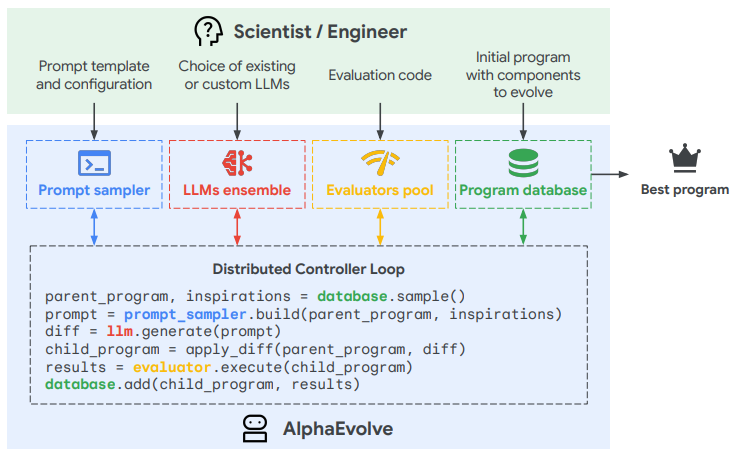
\includegraphics[width=\textwidth]{figures/alpha-evolve.png}
    \caption{The AlphaEvolve program-evolution process, adapted from
    Novikov et al.~\cite{novikov2025alphaevolve}.}
    \label{fig:alpha-evolve}
\end{figure}

\subsection{Task specification and program representation}

An AlphaEvolve task has three essential inputs. First, an initial program must
be complete enough to run, even if its implementation is deliberately simple
(the complete initial program is reproduced in Appendix~\ref{app:initial-program}).
Second, the part of the source code that may be changed is marked with
\texttt{\# EVOLVE-BLOCK-START} and \texttt{\# EVOLVE-BLOCK-END}. The remaining
code forms a fixed skeleton that defines imports, data types, and the public
interface. Third, an evaluator function must be provided. The evaluator
receives the generated program, executes it on the task-specific inputs, and
returns a dictionary of scalar metrics.

\subsection{Prompt sampling and creative generation}

AlphaEvolve prompts contain more than the current program. Depending on the
configuration, the context can contain high-scoring programs, structurally
diverse programs, previous attempts, evaluator outputs, artifacts, explicit
human-written instructions, and relevant examples or literature. The complete
experiment-specific prompt composition is shown in Appendix~\ref{app:prompts-evolution}.
This context allows an LLM to compare alternatives rather than repeatedly
proposing a mutation without knowing what has already been tried.

The LLM is asked to make a concrete source-level change. For a diff-based
mutation, the expected response is a sequence of blocks of the form
\begin{quote}
\texttt{<<<<<<< SEARCH}\\
\texttt{original code}\\
\texttt{=======}\\
\texttt{replacement code}\\
\texttt{>>>>>>> REPLACE}
\end{quote}
The search part identifies the source segment to be replaced, and the replace
part contains the candidate implementation. The complete mutation template is
provided in Appendix~\ref{app:prompt-evolution-user}. A complete rewrite can be used for
short programs or when a targeted change is not appropriate. In both cases,
the model is instructed to preserve the public interface and to optimize the
metrics defined by the evaluator.

AlphaEvolve uses an ensemble rather than relying on only one generation model.
In the original system, a faster model increases the number of explored ideas,
while a more capable model can supply less frequent but more substantial
changes~\cite{novikov2025alphaevolve}. The ensemble is not an ensemble in the
sense of averaging source code. A single model response is selected for each
mutation, after which the resulting program is evaluated independently.

\subsection{Evaluation, evolutionary storage, and distributed execution}

AlphaEvolve supports several mechanisms for making the evaluation stage both
useful and affordable. An evaluation cascade can apply inexpensive tests first
and run expensive tests only for candidates that pass earlier thresholds.
Parallel test cases can be distributed across workers. Multiple
metrics can be returned simultaneously, both because they may represent genuine
objectives and because programs that perform well under different metrics can
provide more varied context for future mutations. Optional LLM feedback can be
used for properties that are difficult to express in a conventional evaluator,
such as readability or simplicity.

The system is implemented as an asynchronous pipeline. LLM generation and
evaluation are started whenever their required inputs are available, and the
controller waits only at dependencies between stages. This maximizes the
number of candidates evaluated within a fixed computation budget instead of
minimizing the latency of an individual candidate.

\subsection{Scope and limitations of AlphaEvolve}

The unique feature of AlphaEvolve is the combination of open-ended LLM
mutations with machine-gradeable selection. It is not a general replacement
for a software engineer, and it cannot be applied directly when candidate
quality cannot be measured by an evaluator. Its results depend on the quality,
coverage, and resistance to exploitation of the evaluation function. A weak
metric can reward a program that optimizes the measurement rather than the
intended task. The search can also require substantial computation because
many candidates must be generated and evaluated, and there is no general
guarantee that the best program will be found within a finite budget.

\section{OpenEvolve}
\label{sec:openevolve}

\subsection{Open-source implementation}

OpenEvolve is an open-source implementation of the AlphaEvolve design~\cite{sharma2025openevolve}
and is used as the execution framework for all surface-realization experiments.
The implementation exposes the same basic interface as AlphaEvolve: an initial
program, an evaluator, and a configuration determine an iterative process in
which programs are proposed, scored, and registered for future use.

The main controller loads the
initial source, initializes the LLM ensemble, prompt sampler, evaluator, and
program database.
The initial program is evaluated before the evolutionary workers are started. On a
fresh run it is then inserted into the database as generation zero. This makes
the baseline available to the selection mechanism and ensures that evolution
starts from a measured candidate rather than an unscored source file.

\subsection{Execution architecture used in the thesis}

The local implementation uses parallel workers for
process-based parallelism. Before a worker is submitted, the controller selects
a parent program and inspiration programs, which are selected the same way as the parent
program, and are used as a source of inspiration for the LLM. Then the controller builds the prompt, calls the LLM,
parses the response, and evaluates the resulting source.

Consequently, the logical evolution loop is:

\begin{enumerate}
  \item select a parent and inspirations;
  \item assemble a prompt from the selected context;
  \item generate and parse an LLM mutation;
  \item execute the candidate evaluator;
  \item register the candidate, metrics, and feedback;
  \item repeat until the iteration budget, target score, or stopping rule is
  reached.
\end{enumerate}

The implementation is asynchronous in practice. Several workers can use
snapshots of the program database made close together, and their results can be incorporated in a
different order from the numerical iteration identifiers. This increases
throughput but means that a candidate does not necessarily use the immediately
preceding candidate as its parent.

\subsection{Extensions made for the experiments}

Several changes were made to the OpenEvolve's algorithm. They address
both the search distribution and the failure modes that are common when a
language model is required to emit an exact source-code patch.

\paragraph{Fitness-weighted and island-specific selection.}
The database was extended with roulette-wheel selection. Parent and inspiration
programs can be sampled with probabilities derived from their fitness instead
of being selected uniformly. A small positive lower bound is used in the
fitness weights so that low-scoring programs are not removed from consideration
immediately. LLM configurations can also be assigned to islands, allowing a
population to be associated with a particular model or model mixture. An
optional iteration-based model schedule was added for periodically forcing a
chosen model.

\paragraph{Configurable inspirations.}
The number of inspiration programs that are selected and added to the prompt can be controlled.

\paragraph{More robust SEARCH/REPLACE application.}
The original exact line matching was extended with trailing-whitespace cleanup
and common-indentation handling. A model can therefore return a source block
with a different outer indentation while the replacement is still inserted at
the correct nesting level. If the response has no parsable diff, a corrective prompt asks the
LLM to return the required format. If a syntactically valid diff does not
change the source because its SEARCH block does not match, a second corrective
prompt includes the parent code and asks the LLM to repair the SEARCH section.
The exact repair prompts are given in Appendix~\ref{app:prompt-repair}.

\paragraph{Retention of failed candidates.}
Malformed or unchanged proposals are written to a separate
directory instead of being silently discarded.
Duplicate source code is detected before insertion.
These changes prevent repeated evaluation of identical candidates and preserve
evidence needed to diagnose the behavior of the LLM and the mutation parser.

\paragraph{Explicit zero scores for timeouts.}
The evaluator integration was changed so that timeout and failed-evaluation
paths give a score of 0.

\section{Program database and initial program}
\label{sec:program-database}

\subsection{Program records and persistence}

The program database is implemented in a way to store those principal fields:

\begin{itemize}
  \item a unique identifier and the program source;
  \item the identifier of the parent program, generation number, timestamp, and
  iteration at which the program was found;
  \item a dictionary of evaluation metrics, including the fitness metric;
  \item derived values such as complexity and diversity and metadata such as
  island assignment and a human-readable change summary;
  \item optional prompts and LLM responses associated with its creation;
  \item optional artifacts and embeddings used for feedback and novelty
  checks.
\end{itemize}

The active database is maintained in memory for fast selection.
For each program, feature coordinates are calculated before insertion.

At most one program is retained as the occupant of a feature cell. If a new
program maps to an empty cell, the cell is occupied. If it maps to an occupied
cell, the program with the better fitness is retained as the cell occupant.
The database separately stores a bounded set of elite programs. The absolute
best program is tracked independently so that it is protected from ordinary
population cleanup. When the configured population limit is exceeded, the
lowest-fitness unprotected programs are removed from the active in-memory
population, together with their references in islands and cells. The main limits are configurable.

\subsection{Initial program}

The initial program, reproduced in Appendix~\ref{app:initial-program}, defines a small \texttt{Triple} data class with
\texttt{subject}, \texttt{predicate}, and \texttt{object} fields. Its evolution
block contains the following baseline behavior: \texttt{predict} receives a
list of triples and returns a
generic sentence for the first triple only:
\begin{quote}
\texttt{The \{predicate\} of \{subject\} is \{object\}.}
\end{quote}
This implementation is intentionally minimal. It
is syntactically valid and satisfies the interface, but it ignores additional
triples, treats every predicate identically, and does not model relations
between entities.

The purpose of evolution is not merely to make this baseline longer. The
desired search direction is from a generic fallback sentence towards a
domain-aware surface realizer. Useful changes include mapping predicates to
natural-language templates, grouping triples by subject, identifying a main
entity, ordering attributes, joining related entities, selecting relative
clauses, and maintaining grammatical agreement. These changes are evaluated
by the generated text rather than being prescribed as a fixed hand-written
algorithm, which allows multiple realization strategies to be explored.

\section{Program selection and prompt engineering}
\label{sec:program-selection}

\subsection{Parent and inspiration selection}

Selection is performed before a worker process is launched. For roulette
selection, the parent is selected from the island using a
fitness-weighted softmax distribution. The use of a distribution
rather than always selecting the best program retains a non-zero probability
of returning to less explored solutions.

Inspirations are selected separately from the parent. They are alternative
programs that can provide a design idea without being the source that is
directly modified. With roulette, their probabilities are
also based on fitness, and the parent itself is excluded from the candidate
inspiration set. The selected parent and inspirations are
passed to the worker, which reconstructs their source code from the database.

\subsection{Prompt composition}

The system message used for the surface-realization experiment is reproduced in
Appendix~\ref{app:prompt-evolution-system}. It contains four kinds of fixed
information:

\begin{itemize}
  \item the role of the model as an expert data engineer;
  \item the description of the data to be processed and the required \texttt{predict} function signature;
  \item an example in which several triples are combined into one complex
  sentence;
  \item the list of predicates that may occur, with one example triple for
  each predicate.
\end{itemize}

The user message is assembled for each selected parent. Its complete template
and runtime components are shown in Appendix~\ref{app:prompt-evolution-user}.
Its main parts are:

\begin{itemize}
  \item the current metrics and fitness score;
  \item optional evaluator artifacts, such as low-scoring triples and the
  generated text that caused them (see Appendix~\ref{app:prompt-artifact-message});
  \item the complete current source code;
  \item the mutation task, including the requirement to improve
  the score, preserve the interface, and use the exact
  SEARCH/REPLACE format.
\end{itemize}

Consequently, the code and score of the selected parent are shown directly in
the current-program section. An inspiration is rendered separately with its
own score and source code. A high-scoring program can therefore provide a
strong implementation pattern, while a structurally different inspiration can
suggest a different way of grouping or ordering triples.

\subsection{SEARCH/REPLACE instructions and their extensions}

The mutation prompt asks for a targeted edit rather than a complete rewritten
file. The SEARCH section must identify source text present in the current
program, and the REPLACE section must contain the proposed replacement. The
controller extracts all matching blocks with a regular expression, applies
them line by line, and checks whether the resulting source differs from the
parent. This format makes changes auditable and reduces the risk that the LLM
rewrites fixed parts of the program unintentionally. The full mutation prompt
is given in Appendix~\ref{app:prompt-evolution-user}.

The format is also a significant source of failure. A model can describe a
patch in prose, omit one of the delimiters, copy an outdated version of the
source, or use an indentation that prevents an exact match. These problems
are adressed in two ways. First, trailing whitespace
is normalized and common indentation is removed while matching, after which
the replacement is re-indented at the original location. Second, malformed
responses and unapplied responses are sent to dedicated repair prompts. These
safeguards preserve the replacement text where possible and focus the subsequent
LLM call on producing a matchable SEARCH section; the repair messages are
listed in Appendix~\ref{app:prompt-repair}.

\section{Large Language Model}
\label{sec:large-language-model}

\subsection{Parsing the LLM response}

OpenEvolve uses an OpenAI-compatible client interface, so the same orchestration
code can communicate with hosted models or local servers. The response is
processed in the worker in the following order:

\begin{enumerate}
  \item The response is searched for one or more SEARCH/REPLACE blocks.
  \item Each block is normalized into source lines and applied to the parent
  source.
  \item If at least one block is found but no source line is changed, the
  response is treated as an unapplied mutation rather than as a successful
  no-op.
  \item A new identifier is assigned and the candidate is passed to the
  evaluator.
\end{enumerate}

When no valid block is found, the response is not immediately treated as a
failed iteration. Up to four attempts are made. The first repair instruction
explains the required delimiter format. If a block was parsed but could not be
applied, the repair instruction additionally contains the original parent code
and asks the model to correct the SEARCH section while preserving the
replacement. The intermediate invalid responses are joined and retained as
diagnostic feedback.

If all repair attempts fail, a child record carrying the unchanged parent code
is returned with an error and a \texttt{no\_valid\_diffs} or \texttt{no\_changes}
artifact. The controller writes this record to the list of broken programs and
does not add it to the active evolutionary population.

OpenEvolve also contains a full-rewrite mode. When diff-based evolution is
disabled, a fenced code block or the plain response is parsed as the complete
candidate source. This mode was retained for compatibility, but the surface
realization experiments use targeted diffs because the evolved function is
embedded in a fixed program skeleton.

\subsection{Invalid programs and execution safety}

A generated program can fail before it produces any text. Dynamic loading can
fail because of a syntax error or missing import; the required \texttt{predict}
function can be absent or have the wrong signature; and a call can return a
non-string value, raise an exception, or run indefinitely. These cases are
converted into zero-valued fitness and artifacts describing the failure rather
than terminating the entire evolution run. The artifacts can then be included
in a later prompt, where they provide a concrete example of what should be
avoided.

\section{Evaluation}
\label{sec:surface-evaluation}

\subsection{Evaluation and feedback}

The OpenEvolve \texttt{Evaluator} is a generic wrapper around the task-specific
evaluation file. For every candidate, it invokes the function named \texttt{evaluate}. The result contain metrics and
artifacts. The wrapper applies the configured timeout, handles
retries, converts both result formats to a common representation, and collects
pending artifacts for the program record.

The initial program is passed through the same evaluator before evolution
starts. This establishes the baseline against which later candidates are
compared. A worker follows the same path after it has applied an LLM mutation.

The task-specific evaluator is therefore the boundary between source-code
generation and evolutionary selection: OpenEvolve does not infer whether a
sentence is good from the source code itself. It returns a metric dictionary and optional \emph{artifacts}, which
are stored diagnostic messages rather than values used directly for ranking.
The metric named \texttt{combined\_score} is the scalar fitness used by the
database. Two mutually exclusive fitness modes are used:

\begin{itemize}
  \item BLEU score evaluation; evaluates reference text with the generated text;
  \item LLM as a judge evaluation; evaluates the generated text with an LLM judge that compares the reference text with the generated text.
\end{itemize}

The code can calculate BLEU in judge-based runs as a diagnostic, but only the
selected mode supplies fitness.

\subsection{Reference-based evaluation}

The surface-realization evaluator loads a supplied reference data corpus.
Each selected entry contains a triple set and one or more reference
lexicalizations.

Before the examples are processed, the evaluator loads the candidate module
dynamically and checks that \texttt{predict} exists and accepts exactly one
argument. For each reference data entry, the list of triples is passed to
\texttt{predict}. A result is accepted only when it is a string. An empty
string receives a per-example zero lexical score. Exceptions, invalid return types, and timeouts terminate the
affected evaluation path and produce zero-valued metrics with an explanation in
the artifacts.

For every non-empty generated text, the evaluator computes a fitness score (which is a BLUE score or LLM as a judge evaluation) against
all reference lexicalizations associated with the entry. The average over the
selected domain entries is returned as an aggregate reference-based measure.

\subsection{Artifacts and continuation}

An artifact is a per-candidate diagnostic message retained alongside its metrics.
In BLEU-driven runs, a low-scoring artifact contains the input triples, generated
text, reference lexicalizations, and the BLEU result. In judge-driven runs, it
contains the triples, generated text, reference text, judge review, and rating.
The worst scored artifacts are retained and three of them are randomly selected for inclusion in the next prompt.

After evaluation, the controller registers the child source, parent identifier,
metrics, and artifacts, updates the population, archive, feature-cell
representative, and best-program record, and submits another iteration. Optional
trace files additionally record this provenance for later inspection. The
repeated sequence of mutation, execution, scoring, and registration is what
turns LLM code generation into the surface-realization search used in this
thesis.


\chapter{Experiments}

\section{Meaning representation}

\subsection{Data Collection}

The experimental evaluation for meaning representation requires structured data
from diverse domains. To obtain such data, \emph{quintd}~\cite{kasner2024beyond}
is used, a framework for collecting \emph{ad hoc} data-to-text datasets. 
Quintd selects examples using
a random seed and can also obtain up-to-date information from external data
sources.

The source collection used in the experiments is denoted by $S_0$. It contains
the five domains available in the corresponding quintd collection: GSMArena,
OpenWeather, Our World in Data (OWID), Wikidata, and ice hockey. The automatic
pipeline comparison uses all five domains. The human evaluation, fine-tuning,
and whole-system experiments use the four-domain subset consisting of GSMArena,
OpenWeather, OWID, and Wikidata. This distinction is important because ice
hockey is included in the automatic pipeline results but is absent from the
later $S_1$, $S_2$, $S_3$, and $S_4$ datasets.

The four experimental datasets are:

\begin{description}
  \item[\textbf{GSMArena}] Mobile phone specifications scraped from the GSMArena
  website. Each instance describes a single phone model with nested categories
  such as Network, Launch, Body, Display, Platform, Memory, Camera, and
  Battery, containing attribute--value pairs.

  \item[\textbf{OpenWeather}] Five-day weather forecasts obtained from the
  OpenWeather API. Each instance contains a time series of 40 three-hour
  intervals, with each interval recording temperature, humidity, wind speed,
  cloud coverage, and weather conditions.

  \item[\textbf{OWID}] Country-level time-series metrics from the Our World in
  Data project. Each instance represents a single metric, such as life
  expectancy, vaccination rates, or reproduction rate, for a specific country
  and contains yearly data points spanning several decades.

  \item[\textbf{Wikidata}] Knowledge-graph entities and their properties from
  Wikidata. Each instance describes an entity, such as a country, film, or
  organization, with a list of property--value pairs such as capital, cast
  member, or language used.
\end{description}

The fifth domain, \emph{ice hockey}, is therefore included only in the automatic
pipeline comparison. Its absence from the human evaluation, fine-tuning, and
whole-system experiments should not be interpreted as an omission from the
source collection.

All experimental datasets are provided as JSON files containing arrays of
structured records. A \emph{raw structured instance} is defined as a single
JSON object representing one self-contained data record from one of the four
experimental domains. Each instance contains nested fields with structured
data---time series, categorical values, numerical measurements, or hierarchical
attribute lists---that must be converted into semantic triples. Let
$D = \{d_1, \dots, d_N\}$ denote the set of $N$ such instances extracted from
the input JSON for a given domain.

\paragraph{Large language model.}
All LLM invocations across the three conversion methods use \emph{Gemma~4
31B IT}~\cite{team2024gemma,team2026gemma}, a 31-billion-parameter
instruction-tuned language model released by Google. The model is served via
\emph{vLLM}~\cite{kwon2023vllm}, a high-throughput inference engine that uses
\emph{PagedAttention} to manage key--value cache memory and enable batched
inference with dynamic sequence lengths.

\subsection{Experimental setup for pipelines}
\label{sec:experimental-setup}

The automatic pipeline comparison uses the $S_0$ source collection of 100 instances from each of the five
experimental domains. The reference-text generation stage is shared by the
three pipelines, while the text-to-triples stage is run separately for
Text-First Extraction with Normalization, Blueprint-Iterative Refinement, and
Evolving Catalog.

The generated outputs are evaluated using a human evaluation and an LLM as a judge. The judge is the
same Gemma~4 31B IT model, but it is used in a separate evaluation role rather
than as part of the extraction pipeline. Two transitions are assessed
independently:

\begin{enumerate}
    \item the conversion from the raw structured instance to the generated
    natural-language reference text; and
    \item the conversion from the reference text to the generated semantic
    triples.
\end{enumerate}

The two transitions use different pairs of criteria, with the complete prompts
provided in Appendix~\ref{app:pipeline-judge-prompts}. The data-to-text
transition is assessed for \emph{summary} and \emph{faithfulness}. Summary
measures whether the generated text is concise, coherent, non-redundant, and
preserves the core message of the structured source. Faithfulness measures
whether every textual claim is supported by that source, penalizing
hallucinations, contradictions, and material distortions. The text-to-triples
transition is assessed for \emph{additions} and \emph{omissions}. Additions
measures whether the triples introduce facts not supported by the reference
text, whereas omissions measures whether they leave out information whose
absence changes meaning, hides important context, or creates a misleading
imbalance. Every criterion is scored on an ordinal scale from 1 to 5, where 5
represents the best result.

The shared data-to-text evaluation requires $5 \times 100 \times 2 = 1{,}000$
judge calls. The three text-to-triples methods require
$5 \times 100 \times 3 \times 2 = 3{,}000$ further calls, for 4,000 calls in
total. For each domain and criterion, scores are averaged over the 100
instances. The resulting averages are used to compare the conversion methods.

The evaluation output also contains descriptive statistics. These statistics
are computed without additional LLM calls and describe the size and structure
of the generated outputs: the number of primitive JSON elements, reference
words, reference sentences, reference subsentences, extracted triples, and
unique predicates. The overall text and triples scores are calculated as the
mean of the two criteria belonging to the corresponding transition.

\begin{table}[!htbp]
\centering
\scriptsize
\caption{Automatic data-to-text evaluation shared by the three pipelines.}
\label{tab:pipeline-text-results}
\begin{tabular}{lrrrr}
\hline
\textbf{Domain} & \textbf{Summary} & \textbf{Faithfulness} & \textbf{Overall} & \textbf{JSON elements} \\
\hline
Ice hockey & 5.000 & 4.950 & 4.970 & 111.67 \\
GSMArena & 5.000 & 5.000 & 5.000 & 111.07 \\
OWID & 4.990 & 4.930 & 4.960 & 478.06 \\
OpenWeather & 5.000 & 5.000 & 5.000 & 902.92 \\
Wikidata & 4.990 & 4.990 & 4.990 & 13.18 \\
\hline
\textbf{Average} & 4.996 & 4.974 & 4.984 & 323.38 \\
\hline
\end{tabular}
\end{table}

\newcommand{\tripleheader}{\textbf{Domain} & \textbf{Additions} & \textbf{Omissions} & \textbf{Overall} & \textbf{Ref. words} & \textbf{Ref. sent.} & \textbf{Ref. subsent.} & \textbf{Triples} & \textbf{Predicates} \\}
\begin{table}[!htbp]
\centering
\scriptsize
\caption{Automatic text-to-triples evaluation for Blueprint-Iterative Refinement.}
\label{tab:pipeline-blueprint-triples-results}
\resizebox{\textwidth}{!}{%
\begin{tabular}{lrrrrrrrr}
\hline
\tripleheader
\hline
Ice hockey & 3.580 & 3.380 & 3.480 & 34.07 & 1.35 & 4.26 & 4.79 & 12 \\
GSMArena & 4.960 & 3.840 & 4.400 & 70.74 & 3.34 & 9.05 & 12.96 & 25 \\
OWID & 4.940 & 4.810 & 4.880 & 57.18 & 2.27 & 6.22 & 15.87 & 8 \\
OpenWeather & 4.880 & 3.840 & 4.360 & 66.21 & 2.82 & 6.53 & 5.46 & 18 \\
Wikidata & 4.910 & 4.410 & 4.660 & 20.34 & 1.17 & 2.61 & 4.15 & 47 \\
\hline
\textbf{Average} & 4.654 & 4.056 & 4.356 & 49.71 & 2.19 & 5.73 & 8.65 & 22.0 \\
\hline
\end{tabular}
}%
\end{table}

\begin{table}[!htbp]
\centering
\scriptsize
\caption{Automatic text-to-triples evaluation for Text-First Extraction with Normalization.}
\label{tab:pipeline-text-first-triples-results}
\resizebox{\textwidth}{!}{%
\begin{tabular}{lrrrrrrrr}
\hline
\tripleheader
\hline
Ice hockey & 5.000 & 4.970 & 4.990 & 32.54 & 1.32 & 4.21 & 6.77 & 106 \\
GSMArena & 5.000 & 5.000 & 5.000 & 70.34 & 3.26 & 9.30 & 13.61 & 159 \\
OWID & 5.000 & 4.990 & 5.000 & 58.23 & 2.28 & 6.31 & 8.09 & 281 \\
OpenWeather & 5.000 & 5.000 & 5.000 & 66.54 & 2.83 & 6.65 & 10.78 & 349 \\
Wikidata & 4.970 & 5.000 & 4.990 & 20.00 & 1.15 & 2.55 & 4.22 & 111 \\
\hline
\textbf{Average} & 4.994 & 4.992 & 4.996 & 49.53 & 2.17 & 5.80 & 8.69 & 201.2 \\
\hline
\end{tabular}
}%
\end{table}

\begin{table}[!htbp]
\centering
\scriptsize
\caption{Automatic text-to-triples evaluation for Evolving Catalog.}
\label{tab:pipeline-catalog-triples-results}
\resizebox{\textwidth}{!}{%
\begin{tabular}{lrrrrrrrr}
\hline
\tripleheader
\hline
Ice hockey & 4.990 & 3.920 & 4.460 & 31.88 & 1.27 & 4.10 & 5.14 & 4 \\
GSMArena & 4.970 & 4.810 & 4.890 & 69.48 & 3.19 & 9.11 & 12.87 & 25 \\
OWID & 4.880 & 3.850 & 4.370 & 56.55 & 2.22 & 5.99 & 3.40 & 139 \\
OpenWeather & 4.830 & 4.320 & 4.580 & 65.62 & 2.77 & 6.77 & 8.84 & 10 \\
Wikidata & 4.810 & 4.780 & 4.790 & 20.19 & 1.14 & 2.62 & 3.69 & 45 \\
\hline
\textbf{Average} & 4.896 & 4.336 & 4.618 & 48.74 & 2.12 & 5.72 & 6.79 & 44.6 \\
\hline
\end{tabular}
}%
\end{table}

\FloatBarrier
\subsection{Human evaluation for pipelines}

Human evaluation follows the same asymmetric rubric as automatic evaluation.
The shared data-to-text transition is assessed for summary and faithfulness,
while each text-to-triples pipeline is assessed for additions and omissions.
For each of the four domains, ten instances are assessed for every relevant
transition. Scores are assigned by the author of the thesis on the same 1--5
scale as automatic evaluation.

\begin{table}[!htbp]
\centering
\caption{Human evaluation of the shared data-to-text transition.}
\label{tab:human-text-results}
\begin{tabular}{lrrr}
\hline
\textbf{Domain} & \textbf{Summary} & \textbf{Faithfulness} & \textbf{Overall} \\
\hline
GSMArena & 4.10 & 3.60 & 3.85 \\
OWID & 4.70 & 4.80 & 4.75 \\
OpenWeather & 4.60 & 3.60 & 4.10 \\
Wikidata & 4.60 & 4.80 & 4.70 \\
\hline
\textbf{Average} & 4.50 & 4.20 & 4.35 \\
\hline
\end{tabular}
\end{table}

\newcommand{\humantripleheader}{\textbf{Domain} & \textbf{Additions} & \textbf{Omissions} & \textbf{Overall} \\}
\begin{table}[!htbp]
\centering
\caption{Human evaluation of Blueprint-Iterative Refinement.}
\label{tab:human-blueprint-results}
\begin{tabular}{lrrr}
\hline
\humantripleheader
\hline
GSMArena & 4.30 & 3.70 & 4.00 \\
OWID & 4.00 & 4.30 & 4.15 \\
OpenWeather & 5.00 & 3.00 & 4.00 \\
Wikidata & 4.80 & 4.30 & 4.55 \\
\hline
\textbf{Average} & 4.525 & 3.825 & 4.175 \\
\hline
\end{tabular}
\end{table}

\begin{table}[!htbp]
\centering
\caption{Human evaluation of Text-First Extraction with Normalization.}
\label{tab:human-text-first-results}
\begin{tabular}{lrrr}
\hline
\humantripleheader
\hline
GSMArena & 4.90 & 5.00 & 4.95 \\
OWID & 5.00 & 4.50 & 4.75 \\
OpenWeather & 4.90 & 5.00 & 4.95 \\
Wikidata & 5.00 & 5.00 & 5.00 \\
\hline
\textbf{Average} & 4.950 & 4.875 & 4.913 \\
\hline
\end{tabular}
\end{table}

\begin{table}[!htbp]
\centering
\caption{Human evaluation of Evolving Catalog.}
\label{tab:human-catalog-results}
\begin{tabular}{lrrr}
\hline
\humantripleheader
\hline
GSMArena & 4.90 & 4.90 & 4.90 \\
OWID & 5.00 & 2.20 & 3.60 \\
OpenWeather & 4.90 & 3.70 & 4.30 \\
Wikidata & 4.80 & 4.80 & 4.80 \\
\hline
\textbf{Average} & 4.900 & 3.900 & 4.400 \\
\hline
\end{tabular}
\end{table}

\FloatBarrier
\subsection{Correlation between LLM and human evaluation}

The agreement between the LLM judge and the human evaluator is computed from
paired 1--5 scores.

The \emph{LLM score mean} and \emph{Human score mean} columns report the
arithmetic mean of the aligned score vector used for that row. For an additions
or omissions row, each mean is calculated from the ten scores for that single
criterion. For a pooled row, it is calculated from 20 scores: additions and
omissions for each of the ten instances. For a per-instance-mean row, it is
calculated from ten instance-level averages. These columns describe the rating
level of each evaluator and are not correlation coefficients.

Four complementary statistics are reported. Pearson's product--moment
correlation measures linear association between the raw values, but assumes
equal distances between the ordinal score levels. Spearman's $\rho$ measures
whether the LLM and human rank instances similarly and is the primary
association measure for the ordinal 1--5 scale. Kendall's $\tau$-b measures
pairwise rank concordance while correcting for ties, making it useful for the
small samples and repeated ratings in this experiment. Quadratic weighted
Cohen's kappa measures chance-corrected ordinal agreement and penalizes a
two-point disagreement more strongly than a one-point disagreement
\cite{cohen1960agreement}. All four measures range from $-1$ to $1$; positive
values indicate agreement or positive association, zero indicates no
association or agreement beyond chance, and negative values indicate inverse
association.

The overall variants are calculated separately for the two evaluation tasks and
never mix data-to-text with text-to-triples. A \emph{pooled} text-to-triples
result concatenates the additions and omissions score of every matched instance
for each rater. With ten matched instances, this produces 20 paired criterion
scores: additions and omissions for each instance. It preserves
criterion-specific disagreement, for example when a judge agrees on additions
but not on omissions.

The complementary \emph{per-instance mean} result first averages additions and
omissions for each rater within an instance and then correlates the resulting
ten overall-quality pairs. It answers whether the LLM and human agree about
which complete instances are better or worse overall, while deliberately
discarding criterion-specific differences. For this mean variant, Pearson,
Spearman, and Kendall are computed from the floating-point means; quadratic
weighted kappa uses the means rounded to the nearest ordinal score.

Pearson, Spearman, and Kendall are undefined when either rater assigns the same
score to every observation. The status column records such constant-vector
cases. Means remain available for comparing score levels, but are not
correlation coefficients. In particular, a kappa of zero in a constant-vector
case indicates no measurable agreement beyond chance under the observed score
distributions; it does not establish that every individual rating disagreed.

\begin{table}[!htbp]
\centering
\scriptsize
\caption{Data-to-text correlation diagnostics ($N=10$ instances per row).}
\label{tab:judge-human-text-correlation}
\resizebox{\textwidth}{!}{%
\begin{tabular}{llrrrrrrl}
\hline
\textbf{Domain} & \textbf{Criterion} & \textbf{Pearson $r$} & \textbf{Spearman $\rho$} & \textbf{Kendall $\tau$} & \textbf{QW-$\kappa$} & \textbf{LLM score mean} & \textbf{Human score mean} & \textbf{Status} \\
\hline
GSMArena & Summary & -- & -- & -- & 0.000 & 5.00 & 4.10 & LLM constant \\
GSMArena & Faithfulness & -- & -- & -- & 0.000 & 5.00 & 3.60 & LLM constant \\
OWID & Summary & -- & -- & -- & 0.000 & 5.00 & 4.70 & LLM constant \\
OWID & Faithfulness & -- & -- & -- & 0.000 & 5.00 & 4.80 & LLM constant \\
OpenWeather & Summary & -- & -- & -- & 0.000 & 5.00 & 4.60 & LLM constant \\
OpenWeather & Faithfulness & -- & -- & -- & 0.000 & 5.00 & 3.60 & LLM constant \\
Wikidata & Summary & -- & -- & -- & 0.000 & 5.00 & 4.60 & LLM constant \\
Wikidata & Faithfulness & -- & -- & -- & 0.000 & 5.00 & 4.80 & LLM constant \\
\hline
\end{tabular}
}%
\end{table}

\begin{table}[!htbp]
\centering
\tiny
\caption{Text-to-triples correlation results by criterion and aggregation.}
\label{tab:judge-human-triples-correlation}
\resizebox{\textwidth}{!}{%
\begin{tabular}{lllrrrrrrrl}
\hline
\textbf{Pipeline} & \textbf{Domain} & \textbf{Criterion / aggregation} & \textbf{$N$} & \textbf{$r$} & \textbf{$\rho$} & \textbf{$\tau$} & \textbf{QW-$\kappa$} & \textbf{LLM score mean} & \textbf{Human score mean} & \textbf{Status} \\
\hline
Blueprint & GSMArena & Additions & 10 & -0.509 & -0.509 & -0.509 & -0.212 & 4.90 & 4.30 & ok \\
 &  & Omissions & 10 & 0.349 & 0.387 & 0.360 & 0.286 & 4.00 & 3.70 & ok \\
 &  & Pooled & 20 & 0.402 & 0.371 & 0.344 & 0.316 & 4.45 & 4.00 & ok \\
 &  & Per-instance mean & 10 & 0.000 & 0.000 & 0.000 & 0.000 & 4.45 & 4.00 & ok \\
 & OWID & Additions & 10 & -- & -- & -- & 0.000 & 5.00 & 4.00 & both constant, different \\
 &  & Omissions & 10 & 0.512 & 0.520 & 0.494 & 0.314 & 4.80 & 4.30 & ok \\
 &  & Pooled & 20 & 0.379 & 0.360 & 0.348 & 0.133 & 4.90 & 4.15 & ok \\
 &  & Per-instance mean & 10 & 0.512 & 0.520 & 0.494 & 0.000 & 4.90 & 4.15 & ok \\
 & OpenWeather & Additions & 10 & -- & -- & -- & 0.000 & 4.70 & 5.00 & Human constant \\
 &  & Omissions & 10 & 0.588 & 0.529 & 0.494 & 0.462 & 3.50 & 3.00 & ok \\
 &  & Pooled & 20 & 0.726 & 0.731 & 0.664 & 0.714 & 4.10 & 4.00 & ok \\
 &  & Per-instance mean & 10 & 0.633 & 0.536 & 0.501 & 0.000 & 4.10 & 4.00 & ok \\
 & Wikidata & Additions & 10 & 0.667 & 0.667 & 0.667 & 0.615 & 4.90 & 4.80 & ok \\
 &  & Omissions & 10 & 0.927 & 0.964 & 0.934 & 0.906 & 4.40 & 4.30 & ok \\
 &  & Pooled & 20 & 0.895 & 0.906 & 0.886 & 0.873 & 4.65 & 4.55 & ok \\
 &  & Per-instance mean & 10 & 0.907 & 0.868 & 0.841 & 0.800 & 4.65 & 4.55 & ok \\
\hline
Text-First & GSMArena & Additions & 10 & -- & -- & -- & 0.000 & 5.00 & 4.90 & LLM constant \\
 &  & Omissions & 10 & -- & -- & -- & 0.000 & 5.00 & 5.00 & both constant, same \\
 &  & Pooled & 20 & -- & -- & -- & 0.000 & 5.00 & 4.95 & LLM constant \\
 &  & Per-instance mean & 10 & -- & -- & -- & 0.000 & 5.00 & 4.95 & LLM constant \\
 & OWID & Additions & 10 & -- & -- & -- & 0.000 & 5.00 & 5.00 & both constant, same \\
 &  & Omissions & 10 & -- & -- & -- & 0.000 & 5.00 & 4.50 & LLM constant \\
 &  & Pooled & 20 & -- & -- & -- & 0.000 & 5.00 & 4.75 & LLM constant \\
 &  & Per-instance mean & 10 & -- & -- & -- & 0.000 & 5.00 & 4.75 & LLM constant \\
 & OpenWeather & Additions & 10 & -- & -- & -- & 0.000 & 5.00 & 4.90 & LLM constant \\
 &  & Omissions & 10 & -- & -- & -- & 0.000 & 5.00 & 5.00 & both constant, same \\
 &  & Pooled & 20 & -- & -- & -- & 0.000 & 5.00 & 4.95 & LLM constant \\
 &  & Per-instance mean & 10 & -- & -- & -- & 0.000 & 5.00 & 4.95 & LLM constant \\
 & Wikidata & Additions & 10 & -- & -- & -- & 0.000 & 5.00 & 5.00 & both constant, same \\
 &  & Omissions & 10 & -- & -- & -- & 0.000 & 5.00 & 5.00 & both constant, same \\
 &  & Pooled & 20 & -- & -- & -- & 0.000 & 5.00 & 5.00 & both constant, same \\
 &  & Per-instance mean & 10 & -- & -- & -- & 0.000 & 5.00 & 5.00 & both constant, same \\
\hline
Catalog & GSMArena & Additions & 10 & -- & -- & -- & 0.000 & 5.00 & 4.90 & LLM constant \\
 &  & Omissions & 10 & 0.667 & 0.667 & 0.667 & 0.615 & 4.80 & 4.90 & ok \\
 &  & Pooled & 20 & 0.444 & 0.444 & 0.444 & 0.444 & 4.90 & 4.90 & ok \\
 &  & Per-instance mean & 10 & 0.375 & 0.375 & 0.375 & 0.375 & 4.90 & 4.90 & ok \\
 & OWID & Additions & 10 & -- & -- & -- & 0.000 & 4.60 & 5.00 & Human constant \\
 &  & Omissions & 10 & 0.867 & 0.917 & 0.875 & 0.404 & 3.60 & 2.20 & ok \\
 &  & Pooled & 20 & 0.604 & 0.630 & 0.578 & 0.559 & 4.10 & 3.60 & ok \\
 &  & Per-instance mean & 10 & 0.627 & 0.795 & 0.707 & 0.043 & 4.10 & 3.60 & ok \\
 & OpenWeather & Additions & 10 & -- & -- & -- & 0.000 & 5.00 & 4.90 & LLM constant \\
 &  & Omissions & 10 & 0.753 & 0.646 & 0.631 & 0.478 & 4.40 & 3.70 & ok \\
 &  & Pooled & 20 & 0.782 & 0.647 & 0.632 & 0.630 & 4.70 & 4.30 & ok \\
 &  & Per-instance mean & 10 & 0.591 & 0.410 & 0.387 & 0.000 & 4.70 & 4.30 & ok \\
 & Wikidata & Additions & 10 & -- & -- & -- & 0.000 & 5.00 & 4.80 & LLM constant \\
 &  & Omissions & 10 & 0.667 & 0.667 & 0.667 & 0.615 & 4.80 & 4.80 & ok \\
 &  & Pooled & 20 & 0.459 & 0.459 & 0.459 & 0.444 & 4.90 & 4.80 & ok \\
 &  & Per-instance mean & 10 & 0.804 & 0.646 & 0.626 & 0.412 & 4.90 & 4.80 & ok \\
\hline
\end{tabular}
}%
\end{table}

\FloatBarrier
\subsection{Experimental setup for fine-tuning}

The fine-tuning experiments are conducted on the same four domains as the
pipeline comparison: GSMArena, OpenWeather, OWID, and Wikidata. The
training-and-validation collection is downloaded using seed $S_1$, while the
held-out test collection is downloaded independently using seed $S_2$.

The raw instances from the $S_1$ and $S_2$ collection are converted into reference text
and semantic triples using the Text-First Extraction with Normalization
pipeline. The aligned text--triple outputs are then used as the targets for a
domain-specific model. For each domain, the resulting examples are split into
80\% training data and 20\% validation data. The $S_2$ collection remains
separate and is used only for the final evaluation of the trained models. This
split prevents the test instances from influencing either model fitting or
training-configuration selection.

The fine-tuned model receives one structured instance and is trained to return
both a natural-language reference and its semantic triples in one JSON output.
The base model is Gemma~4 31B IT, and the adaptation is performed using QLoRA.
The base weights remain frozen, while low-rank adapters are trained in the
language-model attention and feed-forward projections. After training, the
adapters are merged into the base model before evaluation.

\subsection{Training Configuration}

The fine-tuning comparison contains five configurations. The standard baseline
uses three epochs. The \emph{baseline-epoch1} variant keeps the
baseline learning rate, adapter capacity, dropout, and weight decay, but trains
for one epoch. The remaining variants change the learning rate, adapter
capacity, or regularization in order to test their influence on the
domain-specialized models.

All training is performed on NVIDIA A100-SXM4 GPUs with 40~GB of VRAM, using
the PLGrid Athena cluster. The common effective batch size is 16, obtained
from a per-device batch size of 1 and 16 gradient-accumulation steps. The
optimizer is 8-bit paged AdamW, the learning-rate schedule is cosine, and the
compute precision is bfloat16. The base model is loaded using 4-bit NF4
quantization with double quantization.

\begin{table}[!htbp]
\centering
\small
\caption{QLoRA configurations used for fine-tuning.}
\label{tab:qlora-config}
\begin{tabular}{lrrrrrrr}
\hline
\textbf{Configuration} & \textbf{Epochs} & \textbf{LR} & \textbf{Warmup} & \textbf{$r$} & \textbf{$\alpha$} & \textbf{Dropout} & \textbf{Weight decay} \\
\hline
baseline & 3 & $10^{-4}$ & 0.03 & 16 & 32 & 0.05 & 0.00 \\
baseline-epoch1 & 1 & $10^{-4}$ & 0.03 & 16 & 32 & 0.05 & 0.00 \\
low\_lr & 5 & $3\times10^{-5}$ & 0.05 & 16 & 32 & 0.05 & 0.01 \\
higher\_capacity & 3 & $5\times10^{-5}$ & 0.05 & 32 & 64 & 0.05 & 0.01 \\
regularized\_capacity & 5 & $3\times10^{-5}$ & 0.10 & 32 & 64 & 0.10 & 0.01 \\
\hline
\end{tabular}
\end{table}

The LoRA configuration targets all attention and MLP projection matrices in
the language-model backbone (\texttt{q\_proj}, \texttt{k\_proj},
\texttt{v\_proj}, \texttt{o\_proj}, \texttt{gate\_proj}, \texttt{up\_proj},
and \texttt{down\_proj}). A positively scoped module pattern excludes the
vision and audio towers of the multimodal checkpoint. This selects 420 target
modules and approximately 25 million trainable parameters, which is less than
0.1\% of the base model.

The maximum sequence length is adjusted per domain to accommodate the varying
sizes of the raw structured instances while staying within the GPU memory
budget. Wikidata uses 8192 tokens, GSMArena and OWID use 4096 tokens, and
OpenWeather uses 6144 tokens. Instances exceeding the selected maximum are
truncated.

After training, the LoRA adapter weights are combined with the frozen base
model weights to produce a standalone model. This process, computes $W_{\mathrm{final}} = W_0 + \Delta W$ for each adapted layer.
The merged model can be served by the same vLLM infrastructure as the base
model and produces both a natural-language verbalization and the corresponding
semantic triples in a single decode pass.

\FloatBarrier
\subsection{Evaluation of fine-tuned models}

The fine-tuned models are evaluated on the held-out $S_2$ test sets for each
domain. The evaluation compares the generated text with the reference text
using BLEU and METEOR. The generated and reference triples are compared as
sets of subject--predicate--object tuples. Micro-averaged triple precision,
recall, and F1 are computed from the resulting true-positive, false-positive,
and false-negative counts. Predicate adherence measures the proportion of
generated predicates that belong to the predicate catalog used to construct
the targets.

The results are reported for the base model, which is the Gemma 4 before any fine-tuning and separately for the five
fine-tuning configurations.

\newcommand{\finetuneheader}{\textbf{Domain} & \textbf{Text BLEU} & \textbf{Text METEOR} & \textbf{Triple precision} & \textbf{Triple recall} & \textbf{Triple F1} & \textbf{Predicate adherence} \\}

\begin{table}[!htbp]
\centering
\small
\caption{Base-model results on the held-out $S_2$ sets.}
\label{tab:finetune-base-results}
\resizebox{\textwidth}{!}{%
\begin{tabular}{lrrrrrr}
\hline
\finetuneheader
\hline
GSMArena & 0.5621 & 0.7455 & 0.0515 & 0.0413 & 0.0458 & 0.3863 \\
OpenWeather & 0.2574 & 0.4931 & 0.0013 & 0.0010 & 0.0011 & 0.3771 \\
OWID & 0.3919 & 0.6170 & 0.0000 & 0.0000 & 0.0000 & 0.4181 \\
Wikidata & 0.7474 & 0.9032 & 0.0305 & 0.0409 & 0.0349 & 0.3280 \\
\hline
\textbf{Average} & 0.4897 & 0.6897 & 0.0208 & 0.0208 & 0.0205 & 0.3774 \\
\hline
\end{tabular}
}%
\end{table}

\begin{table}[!htbp]
\centering
\small
\caption{Fine-tuned model results for the baseline configuration.}
\label{tab:finetune-baseline-results}
\resizebox{\textwidth}{!}{%
\begin{tabular}{lrrrrrr}
\hline
\finetuneheader
\hline
GSMArena & 0.6245 & 0.8297 & 0.4234 & 0.4411 & 0.4321 & 0.7087 \\
OpenWeather & 0.2121 & 0.4463 & 0.0010 & 0.0005 & 0.0007 & 0.2002 \\
OWID & 0.3096 & 0.5757 & 0.0245 & 0.0227 & 0.0236 & 0.7148 \\
Wikidata & 0.7642 & 0.9087 & 0.5137 & 0.4495 & 0.4795 & 0.6635 \\
\hline
\textbf{Average} & 0.4776 & 0.6901 & 0.2407 & 0.2285 & 0.2340 & 0.5718 \\
\hline
\end{tabular}
}%
\end{table}

\begin{table}[!htbp]
\centering
\small
\caption{Fine-tuned model results for the baseline-epoch1 configuration.}
\label{tab:finetune-baseline-epoch1-results}
\resizebox{\textwidth}{!}{%
\begin{tabular}{lrrrrrr}
\hline
\finetuneheader
\hline
GSMArena & 0.5937 & 0.7969 & 0.2936 & 0.2942 & 0.2939 & 0.8389 \\
OpenWeather & 0.3175 & 0.5430 & 0.0013 & 0.0010 & 0.0011 & 0.3199 \\
OWID & 0.3745 & 0.6355 & 0.0090 & 0.0079 & 0.0084 & 0.6147 \\
Wikidata & 0.7136 & 0.8894 & 0.4103 & 0.1154 & 0.1801 & 0.7479 \\
\hline
\textbf{Average} & 0.4998 & 0.7162 & 0.1786 & 0.1046 & 0.1209 & 0.6304 \\
\hline
\end{tabular}
}%
\end{table}

\begin{table}[!htbp]
\centering
\small
\caption{Fine-tuned model results for the low learning-rate configuration.}
\label{tab:finetune-low-lr-results}
\resizebox{\textwidth}{!}{%
\begin{tabular}{lrrrrrr}
\hline
\finetuneheader
\hline
GSMArena & 0.6399 & 0.8257 & 0.3645 & 0.3615 & 0.3630 & 0.7522 \\
OpenWeather & 0.3068 & 0.5421 & 0.0016 & 0.0010 & 0.0012 & 0.3033 \\
OWID & 0.3877 & 0.6457 & 0.0088 & 0.0078 & 0.0083 & 0.6047 \\
Wikidata & 0.7752 & 0.9104 & 0.4363 & 0.4531 & 0.4446 & 0.7280 \\
\hline
\textbf{Average} & 0.5274 & 0.7310 & 0.2028 & 0.2059 & 0.2043 & 0.5971 \\
\hline
\end{tabular}
}%
\end{table}

\begin{table}[!htbp]
\centering
\small
\caption{Fine-tuned model results for the higher-capacity configuration.}
\label{tab:finetune-higher-capacity-results}
\resizebox{\textwidth}{!}{%
\begin{tabular}{lrrrrrr}
\hline
\finetuneheader
\hline
GSMArena & 0.6332 & 0.8316 & 0.4202 & 0.4310 & 0.4256 & 0.7306 \\
OpenWeather & 0.2448 & 0.4786 & 0.0027 & 0.0015 & 0.0019 & 0.1636 \\
OWID & 0.3654 & 0.6276 & 0.0256 & 0.0240 & 0.0248 & 0.6911 \\
Wikidata & 0.7513 & 0.9019 & 0.4757 & 0.4700 & 0.4728 & 0.6971 \\
\hline
\textbf{Average} & 0.4987 & 0.7099 & 0.2311 & 0.2316 & 0.2313 & 0.5706 \\
\hline
\end{tabular}
}%
\end{table}

\begin{table}[!htbp]
\centering
\small
\caption{Fine-tuned model results for the regularized-capacity configuration.}
\label{tab:finetune-regularized-capacity-results}
\resizebox{\textwidth}{!}{%
\begin{tabular}{lrrrrrr}
\hline
\finetuneheader
\hline
GSMArena & 0.6443 & 0.8297 & 0.3961 & 0.3953 & 0.3957 & 0.7373 \\
OpenWeather & 0.2957 & 0.5449 & 0.0025 & 0.0015 & 0.0018 & 0.2789 \\
OWID & 0.3911 & 0.6407 & 0.0191 & 0.0169 & 0.0179 & 0.6858 \\
Wikidata & 0.7555 & 0.8963 & 0.4912 & 0.4700 & 0.4803 & 0.6884 \\
\hline
\textbf{Average} & 0.5217 & 0.7279 & 0.2272 & 0.2209 & 0.2239 & 0.5976 \\
\hline
\end{tabular}
}%
\end{table}

\FloatBarrier
\section{Surface realization}

\subsection{WebNLG dataset and evaluation protocol}

Surface realization is evaluated on WebNLG, a benchmark in which RDF-style
semantic triples are paired with one or more natural-language lexicalizations.
The benchmark reader used in this work loads the English WebNLG release and
preserves both the triples and their reference texts. During evolution, the
training portion of WebNLG is used to provide fitness feedback. The final
programs are evaluated independently on the held-out test portion, preventing
the test references from being used during program search
\cite{gardent-etal-2017-webnlg}.

The evaluation is performed separately by WebNLG domain. The program receives
only the triples for each test entry. It must return one natural-language
string. The baseline systems are a rule-based generator by Lango et al.~~\cite{lango-dusek-2025-llm}, a fine-tuned BART
model, and a prompted language model. The prompt can be found in
Appendix~\ref{app:prompt-llm-judge}.

The final evaluation reports reference-based, judge-based, and descriptive
metrics. BLEU, BLEURT, and METEOR compare a generated text with the WebNLG
references. SENLEN measures the absolute difference between the number of
sentences in the generated text and the average number in the references. The
three judge columns contain scores from Gemma~4 31B IT, Qwen~3.6, and Themis.
The grammaticality, additions, and omissions judgments are performed with
Gemma~4 31B IT. The prompts used for these judgments are provided in
Appendix~\ref{app:prompt-llm-judge}. The final four columns are descriptive
statistics: average sentence count, word count, character count, and number
of input triples.

Higher values are preferable for BLEU, BLEURT, METEOR, judge scores, and
grammaticality. Lower values are preferable for additions, and
omissions; zero means that no addition or
omission was detected. Lower SENLEN values are preferable; zero indicates that
the period-delimited segment count exactly matches the average reference count.

\subsection{Evolution variants}

The initial all-domain run uses 1,000 iterations, Gemma~4 31B IT as the main
program-generation model, BLEU fitness, and one inspiration program in each
prompt. The later runs use 500 or 100 iterations and are restricted to three selected
domains.

The initial run was used to identify domains with different levels of
difficulty. WrittenWork was selected as the best-working domain, Building as
an intermediate domain, and Food as the most difficult domain. Restricting
subsequent variants to these three domains reduced the computational cost
of the experiments while retaining distinct task difficulties.

The following 500-iteration variants were then evaluated:

\begin{description}
    \item[BLEU without inspirations] BLEU fitness and no inspiration programs.
    \item[BLEU with inspirations] BLEU fitness and inspiration programs.
    \item[LLM judge without inspirations] LLM-as-a-judge fitness and no
    inspiration programs.
    \item[LLM judge with inspirations] LLM-as-a-judge fitness and inspiration
    programs.
    \item[Mixed-model LLM judge] LLM-as-a-judge fitness and inspirations, with
    Gemma~4 31B used for 80\% of calls and a 753B model for 20\% of calls.
    \item[Mixed-model LLM judge with four threads] The preceding mixed-model
    setup with four parallel evaluator threads.
\end{description}

Each run produces an executable surface-realization program. The program is
then evaluated on the held-out WebNLG test set rather than being judged only
by its online evolutionary fitness.

\subsection{Evolution results}

The following tables use the metric order shown in the evaluation protocol.
Average rows are calculated over the available rows for the
corresponding experiment.

\newcommand{\surfaceHeader}{\texttt{domain} & \texttt{BLEU} & \texttt{BLEURT} & \texttt{METEOR} & \texttt{SENLEN} & \texttt{Gemma} & \texttt{Qwen} & \texttt{Themis} & \texttt{gram.} & \texttt{add.} & \texttt{om.} & \texttt{sent.} & \texttt{words} & \texttt{chars} & \texttt{triples} \\\hline}
\newcommand{\surfacerow}[9]{#1 & #2 & #3 & #4 & #5 & #6 & #7 & #8 & #9 & \surfacetail}
\newcommand{\surfacetail}[6]{#1 & #2 & #3 & #4 & #5 & #6 \\\hline}
\newcommand{\surfacebaselinerow}[9]{#1 & #2 & #3 & #4 & #5 & #6 & #7 & #8 & #9 & \surfacebaselinetail}
\newcommand{\surfacebaselinetail}[7]{#1 & #2 & #3 & #4 & #5 & #6 & #7 \\\hline}

\begin{table}[!htbp]
\centering\tiny\setlength{\tabcolsep}{1pt}
\caption{Initial BLEU-based evolution variant with one inspiration.}
\label{tab:surface-base}
\begin{tabular}{l*{14}{r}}\hline
\surfaceHeader
\surfacerow{Airport}{0.4125}{0.2992}{0.7108}{0.4649}{0.9053}{0.7179}{0.8421}{0.3789}{0.0737}{0.0000}{0}{0}{0}{0}
\surfacerow{Artist}{0.3006}{0.1340}{0.6203}{0.2661}{0.8239}{0.6936}{0.7725}{0.5872}{0.0092}{0.2018}{0}{0}{0}{0}
\surfacerow{Astronaut}{0.5300}{0.2160}{0.7394}{0.4858}{0.9463}{0.7561}{0.8780}{0.6463}{0.0366}{0.0366}{0}{0}{0}{0}
\surfacerow{Athlete}{0.5632}{0.4583}{0.7828}{0.3000}{0.9360}{0.8280}{0.9240}{0.8200}{0.1000}{0.0000}{0}{0}{0}{0}
\surfacerow{Building}{0.4220}{0.0381}{0.6245}{0.8043}{0.9913}{0.8652}{0.9348}{0.5870}{0.0217}{0.0000}{0}{0}{0}{0}
\surfacerow{CelestialBody}{0.4962}{0.3329}{0.7172}{0.4898}{1.0000}{0.8286}{0.9510}{0.6122}{0.0000}{0.0000}{0}{0}{0}{0}
\surfacerow{City}{0.3463}{0.1817}{0.6536}{0.3976}{0.7831}{0.6843}{0.9157}{0.8072}{0.4578}{0.0000}{0}{0}{0}{0}
\surfacerow{ComicsCharacter}{0.2947}{-0.0221}{0.5241}{0.5500}{0.8000}{0.6067}{0.7733}{0.3000}{0.0000}{0.5667}{0}{0}{0}{0}
\surfacerow{Company}{0.4901}{0.2592}{0.7370}{0.3788}{0.9576}{0.7818}{0.9152}{0.5758}{0.0909}{0.0000}{0}{0}{0}{0}
\surfacerow{Food}{0.0764}{0.0417}{0.5173}{0.8587}{0.8652}{0.4913}{0.6348}{0.0000}{0.0435}{0.0000}{0}{0}{0}{0}
\surfacerow{MeanOfTransportation}{0.3523}{0.2908}{0.7313}{0.2126}{0.9241}{0.7517}{0.8966}{0.5517}{0.0345}{0.0345}{0}{0}{0}{0}
\surfacerow{Monument}{0.4950}{0.2289}{0.6997}{0.8877}{0.6043}{0.4261}{0.6652}{0.3913}{0.5870}{0.0000}{0}{0}{0}{0}
\surfacerow{Politician}{0.5059}{-0.0405}{0.7218}{0.7701}{1.0000}{0.8138}{0.9103}{0.1724}{0.0000}{0.0000}{0}{0}{0}{0}
\surfacerow{SportsTeam}{0.4638}{0.1271}{0.7756}{0.7992}{0.7818}{0.4773}{0.8136}{0.4545}{0.1136}{0.0000}{0}{0}{0}{0}
\surfacerow{University}{0.5473}{0.1314}{0.7261}{0.2926}{0.8733}{0.7889}{0.8644}{0.4444}{0.0889}{0.0111}{0}{0}{0}{0}
\surfacerow{WrittenWork}{0.5920}{0.2027}{0.7628}{0.3488}{0.9907}{0.8326}{0.9535}{0.5116}{0.0000}{0.0000}{0}{0}{0}{0}
\hline
\surfacerow{\textbf{Average}}{0.4305}{0.1800}{0.6903}{0.5192}{0.8864}{0.7090}{0.8528}{0.4900}{0.1036}{0.0532}{0}{0}{0}{0}
\end{tabular}
\end{table}

\begin{table}[!htbp]
\centering\tiny\setlength{\tabcolsep}{1pt}
\caption{BLEU-based evolution without inspirations, Gemma~4 31B, 500 iterations.}
\label{tab:surface-bleu-no-inspirations}
\begin{tabular}{l*{14}{r}}\hline
\surfaceHeader
\surfacerow{WrittenWork}{0.5565}{0.2162}{0.7654}{0.3488}{0.9814}{0.8930}{0.9581}{0.7442}{0.0000}{0.0000}{2.3488}{19.8140}{108.6744}{2.3488}
\surfacerow{Building}{0.4158}{0.0302}{0.6181}{0.8043}{0.9435}{0.7913}{0.8957}{0.3478}{0.1739}{0.0000}{3.3478}{34.7391}{196.8478}{4.5652}
\surfacerow{Food}{0.0841}{0.0683}{0.5106}{0.8587}{0.8609}{0.5087}{0.6913}{0.0000}{0.0435}{0.0000}{1.0000}{26.7609}{156.7391}{4.5652}
\hline
\surfacerow{\textbf{Average}}{0.3521}{0.1049}{0.6314}{0.6706}{0.9286}{0.7310}{0.8484}{0.3640}{0.0725}{0.0000}{2.2322}{27.1047}{154.0871}{3.8264}
\end{tabular}
\end{table}

\begin{table}[!htbp]
\centering\tiny\setlength{\tabcolsep}{1pt}
\caption{BLEU-based evolution with inspirations, Gemma~4 31B, 500 iterations.}
\label{tab:surface-bleu-with-inspirations}
\begin{tabular}{l*{14}{r}}\hline
\surfaceHeader
\surfacerow{WrittenWork}{0.5579}{0.1871}{0.7657}{0.4186}{0.9442}{0.7581}{0.9395}{0.4884}{0.0465}{0.0000}{2.4186}{19.3953}{107.3488}{2.3488}
\surfacerow{Building}{0.4158}{0.0302}{0.6181}{0.8043}{0.9652}{0.8609}{0.8783}{0.3478}{0.1522}{0.0435}{3.3478}{34.7391}{196.8478}{4.5652}
\surfacerow{Food}{0.0841}{0.0683}{0.5106}{0.8587}{0.8478}{0.4913}{0.7043}{0.0000}{0.1304}{0.0000}{1.0000}{26.7609}{156.7391}{4.5652}
\hline
\surfacerow{\textbf{Average}}{0.3526}{0.0952}{0.6315}{0.6939}{0.9191}{0.7034}{0.8407}{0.2787}{0.1097}{0.0145}{2.2555}{26.9651}{153.6453}{3.8264}
\end{tabular}
\end{table}

\begin{table}[!htbp]
\centering\tiny\setlength{\tabcolsep}{1pt}
\caption{LLM-judge evolution without inspirations, Gemma~4 31B, 500 iterations.}
\label{tab:surface-llm-no-inspirations}
\begin{tabular}{l*{14}{r}}\hline
\surfaceHeader
\surfacerow{WrittenWork}{0.5192}{0.2417}{0.7355}{0.4186}{1.0000}{0.9116}{0.9907}{0.9535}{0.0000}{0.0000}{2.4186}{20.4419}{106.9302}{2.3488}
\surfacerow{Building}{0.4198}{0.0804}{0.6118}{0.8043}{1.0000}{0.8087}{0.9043}{0.5870}{0.0000}{0.0000}{3.3478}{37.9565}{203.5435}{4.5652}
\surfacerow{Food}{0.0904}{-0.1788}{0.5009}{0.8587}{1.0000}{0.6435}{0.8435}{0.9348}{0.0000}{0.0000}{1.0000}{26.1522}{153.6739}{4.5652}
\hline
\surfacerow{\textbf{Average}}{0.3431}{0.0478}{0.6161}{0.6939}{1.0000}{0.7879}{0.9128}{0.8251}{0.0000}{0.0000}{2.2555}{28.1835}{154.7159}{3.8264}
\end{tabular}
\end{table}

\begin{table}[!htbp]
\centering\tiny\setlength{\tabcolsep}{1pt}
\caption{LLM-judge evolution with inspirations, Gemma~4 31B, 500 iterations.}
\label{tab:surface-llm-with-inspirations}
\begin{tabular}{l*{14}{r}}\hline
\surfaceHeader
\surfacerow{WrittenWork}{0.5405}{0.2194}{0.7667}{0.3488}{1.0000}{0.9511}{0.9904}{0.8733}{0.0000}{0.0000}{2.3488}{19.8140}{108.6744}{2.3488}
\surfacerow{Building}{0.4168}{0.0214}{0.6231}{0.8043}{1.0000}{0.8783}{0.9565}{0.5870}{0.0000}{0.0000}{3.3478}{34.7391}{196.8478}{4.5652}
\surfacerow{Food}{0.0671}{-0.2275}{0.4968}{0.8587}{0.7391}{0.4174}{0.5739}{0.0435}{0.0435}{0.0000}{1.0000}{27.2609}{157.1739}{4.5652}
\hline
\surfacerow{\textbf{Average}}{0.3414}{0.0044}{0.6289}{0.6706}{0.9130}{0.7489}{0.8403}{0.5013}{0.0145}{0.0000}{2.2322}{27.2713}{154.2321}{3.8264}
\end{tabular}
\end{table}

\begin{table}[!htbp]
\centering\tiny\setlength{\tabcolsep}{1pt}
\caption{Mixed-model LLM-judge evolution with inspirations, 100 iterations.}
\label{tab:surface-llm-mixed}
\begin{tabular}{l*{14}{r}}\hline
\surfaceHeader
\surfacerow{WrittenWork}{0.5499}{0.2371}{0.7615}{0.3488}{1.0000}{0.9721}{0.9953}{0.8837}{0.0000}{0.0000}{2.3488}{20.3721}{110.7907}{2.3488}
\surfacerow{Building}{0.3665}{0.0739}{0.6052}{0.8043}{1.0000}{0.8000}{0.9478}{0.8261}{0.0000}{0.0000}{3.3478}{38.5652}{212.0870}{4.5652}
\surfacerow{Food}{0.0938}{-0.0887}{0.4803}{0.8587}{1.0000}{0.5783}{0.8696}{0.3913}{0.0000}{0.0000}{1.0000}{28.2826}{170.1087}{4.5652}
\hline
\surfacerow{\textbf{Average}}{0.3367}{0.0741}{0.6156}{0.6706}{1.0000}{0.7835}{0.9376}{0.7004}{0.0000}{0.0000}{2.2322}{29.0733}{164.3288}{3.8264}
\end{tabular}
\end{table}

\begin{table}[!htbp]
\centering\tiny\setlength{\tabcolsep}{1pt}
\caption{Mixed-model LLM-judge evolution with inspirations and four threads, 100 iterations.}
\label{tab:surface-llm-mixed-four-threads}
\begin{tabular}{l*{14}{r}}\hline
\surfaceHeader
\surfacerow{WrittenWork}{0.5348}{0.2359}{0.7386}{0.4186}{1.0000}{0.9349}{0.9953}{0.8837}{0.0000}{0.0000}{2.4186}{19.8605}{104.6744}{2.3488}
\surfacerow{Building}{0.3664}{0.0301}{0.6198}{0.8043}{1.0000}{0.7870}{0.9217}{0.9565}{0.0000}{0.0000}{3.3478}{37.9565}{208.8478}{4.5652}
\surfacerow{Food}{0.0721}{-0.1559}{0.4824}{0.8587}{1.0000}{0.7565}{0.9174}{0.6087}{0.0000}{0.0000}{1.0000}{28.8043}{166.3478}{4.5652}
\hline
\surfacerow{\textbf{Average}}{0.3244}{0.0367}{0.6136}{0.6939}{1.0000}{0.8261}{0.9448}{0.8163}{0.0000}{0.0000}{2.2555}{28.8738}{159.9567}{3.8264}
\end{tabular}
\end{table}

\subsection{Configured experiments with unavailable results}

The following configurations were prepared after the runs reported above. They
use no inspiration programs and Gemma~4 31B IT as the LLM judge. Their result
artifacts were not available when this thesis was prepared. Each table is kept
as an explicit zero-filled placeholder so that the experimental matrix and its
intended reporting schema are documented; these zeros are not measured scores.

\newcommand{\surfaceplaceholderbody}{%
\surfacerow{WrittenWork}{0}{0}{0}{0}{0}{0}{0}{0}{0}{0}{0}{0}{0}{0}
\surfacerow{Building}{0}{0}{0}{0}{0}{0}{0}{0}{0}{0}{0}{0}{0}{0}
\surfacerow{Food}{0}{0}{0}{0}{0}{0}{0}{0}{0}{0}{0}{0}{0}{0}
\hline
\surfacerow{\textbf{Average}}{0}{0}{0}{0}{0}{0}{0}{0}{0}{0}{0}{0}{0}{0}}

\begin{table}[!htbp]
\centering\tiny\setlength{\tabcolsep}{1pt}
\caption{Configured 100-iteration mixed Gemma run: 80\% standard generation, 20\% high-reasoning generation, four evaluator threads (\texttt{6\_2gemmas\_thinking\_4thread\_pp}). Results unavailable.}
\label{tab:surface-config-6-two-gemma-four-thread}
\begin{tabular}{l*{14}{r}}\hline
\surfaceHeader
\surfaceplaceholderbody
\end{tabular}
\end{table}

\begin{table}[!htbp]
\centering\tiny\setlength{\tabcolsep}{1pt}
\caption{Configured 100-iteration mixed Gemma run: 80\% standard generation, 20\% high-reasoning generation, one evaluator thread (\texttt{6\_2gemmas\_thinking\_1thread\_pp}). Results unavailable.}
\label{tab:surface-config-6-two-gemma-one-thread-pp}
\begin{tabular}{l*{14}{r}}\hline
\surfaceHeader
\surfaceplaceholderbody
\end{tabular}
\end{table}

\begin{table}[!htbp]
\centering\tiny\setlength{\tabcolsep}{1pt}
\caption{Configured PLGrid 100-iteration mixed Gemma run: 80\% standard generation, 20\% high-reasoning generation, one evaluator thread (\texttt{6\_2gemmas\_thinking\_1thread\_plgrid}). Results unavailable.}
\label{tab:surface-config-6-two-gemma-one-thread-plgrid}
\begin{tabular}{l*{14}{r}}\hline
\surfaceHeader
\surfaceplaceholderbody
\end{tabular}
\end{table}

\begin{table}[!htbp]
\centering\tiny\setlength{\tabcolsep}{1pt}
\caption{Configured 500-iteration high-reasoning Gemma~4 31B run with four evaluator threads (\texttt{6\_1gemma\_thinking\_4thread\_500iter\_pp}). Results unavailable.}
\label{tab:surface-config-6-one-gemma-thinking}
\begin{tabular}{l*{14}{r}}\hline
\surfaceHeader
\surfaceplaceholderbody
\end{tabular}
\end{table}

\begin{table}[!htbp]
\centering\tiny\setlength{\tabcolsep}{1pt}
\caption{Configured 500-iteration Gemma~4 E4B run with one evaluator thread (\texttt{7\_gemma\_1thread\_500iter\_pp}). Results unavailable.}
\label{tab:surface-config-7-gemma}
\begin{tabular}{l*{14}{r}}\hline
\surfaceHeader
\surfaceplaceholderbody
\end{tabular}
\end{table}

\begin{table}[!htbp]
\centering\tiny\setlength{\tabcolsep}{1pt}
\caption{Configured 500-iteration Llama~3.3 70B Instruct AWQ INT4 run with one evaluator thread (\texttt{7\_llama\_1thread\_500iter\_pp}). Results unavailable.}
\label{tab:surface-config-7-llama}
\begin{tabular}{l*{14}{r}}\hline
\surfaceHeader
\surfaceplaceholderbody
\end{tabular}
\end{table}

\begin{table}[!htbp]
\centering\tiny\setlength{\tabcolsep}{1pt}
\caption{Configured 500-iteration Qwen3 32B AWQ run with one evaluator thread (\texttt{7\_qwen\_1thread\_500iter\_pp}). Results unavailable.}
\label{tab:surface-config-7-qwen}
\begin{tabular}{l*{14}{r}}\hline
\surfaceHeader
\surfaceplaceholderbody
\end{tabular}
\end{table}

\begin{table}[!htbp]
\centering\tiny\setlength{\tabcolsep}{1pt}
\caption{Configured 500-iteration standard Gemma~4 31B run with one evaluator thread (\texttt{8\_1gemma\_noref\_1thread\_500\_iter\_pp}). Results unavailable.}
\label{tab:surface-config-8-gemma-no-reasoning}
\begin{tabular}{l*{14}{r}}\hline
\surfaceHeader
\surfaceplaceholderbody
\end{tabular}
\end{table}

\FloatBarrier
\subsection{Baseline systems}

The baselines are a rule-based generator, a fine-tuned BART model, and an LLM
prompt. The average is calculated over the available domain results for each
baseline.

\begin{table}[!htbp]
\centering\tiny\setlength{\tabcolsep}{1pt}
\caption{Baseline scores across WebNLG domains.}
\label{tab:surface-baselines}
\resizebox{\textwidth}{!}{%
\begin{tabular}{ll*{14}{r}}\hline
\texttt{method} & \texttt{domain} & \texttt{BLEU} & \texttt{BLEURT} & \texttt{METEOR} & \texttt{SENLEN} & \texttt{Gemma} & \texttt{Qwen} & \texttt{Themis} & \texttt{gram.} & \texttt{add.} & \texttt{om.} & \texttt{sent.} & \texttt{words} & \texttt{chars} & \texttt{triples} \\\hline
\surfacebaselinerow{Rule-based generator}{all domains}{0.1702}{-0.3874}{0.5205}{1.0175}{0.4108}{0.4811}{0.7552}{0.1783}{0.0889}{0.0742}{2.5414}{21.7471}{146.6654}{3.1946}
\surfacebaselinerow{Fine-tuned BART}{all domains}{0.5077}{0.2599}{0.7163}{0.5157}{0.6366}{0.5933}{0.7899}{0.8366}{0.3142}{0.1863}{2.1679}{138.9440}{23.7167}{3.5205}
\surfacebaselinerow{LLM prompt}{all domains}{0.5019}{0.3443}{0.7246}{0.5274}{0.9954}{0.9743}{0.9847}{0.9861}{0.0045}{0.0022}{1.7307}{132.0601}{21.5757}{3.5205}
\hline
\end{tabular}
}%
\end{table}

\FloatBarrier
\subsection{Three-domain comparison}

The final comparison reports averages over WrittenWork, Building, and Food for
the baselines and all six reported three-domain OpenEvolve variants. The
all-domain initial variant is omitted because descriptive statistics were not
reported for that run.

\begin{table}[!htbp]
\centering\tiny\setlength{\tabcolsep}{1pt}
\caption{Average scores on WrittenWork, Building, and Food.}
\label{tab:surface-final-comparison}
\resizebox{\textwidth}{!}{%
\begin{tabular}{l*{14}{r}}\hline
\texttt{method} & \texttt{BLEU} & \texttt{BLEURT} & \texttt{METEOR} & \texttt{SENLEN} & \texttt{Gemma} & \texttt{Qwen} & \texttt{Themis} & \texttt{gram.} & \texttt{add.} & \texttt{om.} & \texttt{sent.} & \texttt{words} & \texttt{chars} & \texttt{triples} \\\hline
\surfacerow{Rule-based generator}{0.2063}{-0.4489}{0.5498}{1.9138}{0.2316}{0.3529}{0.6380}{0.0694}{0.4291}{0.1836}{4.3887}{30.8329}{199.2032}{3.3999}
\surfacerow{Fine-tuned BART}{0.5628}{0.2398}{0.7126}{0.7414}{0.6707}{0.5964}{0.8123}{0.7878}{0.2782}{0.1122}{2.3025}{147.8967}{27.3637}{3.8264}
\surfacerow{LLM prompt}{0.4781}{0.2310}{0.6720}{0.6706}{0.9848}{0.9660}{0.9826}{0.9778}{0.0000}{0.0000}{2.2322}{141.2164}{25.2174}{3.8264}
\hline
\surfacerow{BLEU, no inspirations}{0.3521}{0.1049}{0.6314}{0.6706}{0.9286}{0.7310}{0.8484}{0.3640}{0.0725}{0.0000}{2.2322}{27.1047}{154.0871}{3.8264}
\surfacerow{BLEU, with inspirations}{0.3526}{0.0952}{0.6315}{0.6939}{0.9191}{0.7034}{0.8407}{0.2787}{0.1097}{0.0145}{2.2555}{26.9651}{153.6453}{3.8264}
\surfacerow{LLM judge, no inspirations}{0.3431}{0.0478}{0.6161}{0.6939}{1.0000}{0.7879}{0.9128}{0.8251}{0.0000}{0.0000}{2.2555}{28.1835}{154.7159}{3.8264}
\surfacerow{LLM judge, with inspirations}{0.3414}{0.0044}{0.6289}{0.6706}{0.9130}{0.7489}{0.8403}{0.5013}{0.0145}{0.0000}{2.2322}{27.2713}{154.2321}{3.8264}
\surfacerow{Mixed-model LLM judge}{0.3367}{0.0741}{0.6156}{0.6706}{1.0000}{0.7835}{0.9376}{0.7004}{0.0000}{0.0000}{2.2322}{29.0733}{164.3288}{3.8264}
\surfacerow{Mixed-model LLM judge, 4 threads}{0.3244}{0.0367}{0.6136}{0.6939}{1.0000}{0.8261}{0.9448}{0.8163}{0.0000}{0.0000}{2.2555}{28.8738}{159.9567}{3.8264}
\end{tabular}
}%
\end{table}


\FloatBarrier
\section{Whole system evaluation}

The whole-system evaluation combines the meaning-representation and surface-
realization stages into one experimental pipeline. Unlike the preceding
experiments, which evaluate the two stages separately, this evaluation measures
whether errors introduced while converting raw structured data into triples
affect the final generated text.

\subsection{Data construction}

Two new collections are downloaded with quintd for each of the four domains:
GSMArena, OpenWeather, OWID, and Wikidata. The first collection is denoted by
$S_3$ and contains 1,000 raw structured instances per domain for training the
evolutionary programs. The second collection is denoted by $S_4$ and contains
another 1,000 raw structured instances per domain for final testing. The two
collections are downloaded independently so that no raw instance from the test
collection is available during evolution.

The raw instances in both collections are processed with the \emph{regularized capacity}
fine-tuned Gemma~4 model from the preceding fine-tuning experiments. For each
instance, the model produces a natural-language reference and the associated
normalized semantic triples in a single output. Thus, both $S_3$ and $S_4$
contain aligned pairs of the form
\[
    (T_i, r_i),
\]
where $T_i$ is the generated set of triples and $r_i$ is the corresponding
reference text. The model is selected before this evaluation and remains frozen
while the whole-system experiments are performed. The generated references are
therefore used as domain-specific evaluation targets, rather than as additional
inputs to the surface-realization programs.

\subsection{Evolution and evaluation protocol}

For each domain, the selected best-working OpenEvolve variant is run using the
$S_3$ collection. The evolved program receives only $T_i$ and must generate a
natural-language text. Its fitness is computed by comparing the generated text
with $r_i$ on the 1,000 training instances. A separate best program is retained
for each domain. The $S_4$ triples and reference texts are not used during
program generation, fitness calculation, or program selection.

After evolution, each domain-specific program is executed on all 1,000
instances in the corresponding $S_4$ test collection. The generated texts are
evaluated using the same protocol as the WebNLG surface-realization
experiments. BLEU, BLEURT, and METEOR compare the generated text with its
reference. SENLEN measures the difference between the generated and reference
sentence counts. Gemma~4, Qwen, and Themis provide judge scores, while
grammaticality, additions, and omissions are evaluated using the corresponding
judge prompts. Average sentence count, word count, character count, and number
of input triples are reported as descriptive statistics.

In this experiment, the reference triples are produced by the selected
fine-tuned model rather than annotated independently by humans. Consequently,
the evaluation measures the quality of the complete data-to-text pipeline with
respect to the distilled references. It does not separately estimate the
semantic precision or recall of the fine-tuned model; those properties are
reported in the fine-tuning experiments.

\begin{table}[!htbp]
\centering\tiny\setlength{\tabcolsep}{1pt}
\caption{Whole-system evaluation on the independent $S_4$ test collections.}
\label{tab:whole-system-results}
\begin{tabular}{l*{14}{r}}\hline
\surfaceHeader
\surfacerow{GSMArena}{0}{0}{0}{0}{0}{0}{0}{0}{0}{0}{0}{0}{0}{0}
\surfacerow{OpenWeather}{0}{0}{0}{0}{0}{0}{0}{0}{0}{0}{0}{0}{0}{0}
\surfacerow{OWID}{0}{0}{0}{0}{0}{0}{0}{0}{0}{0}{0}{0}{0}{0}
\surfacerow{Wikidata}{0}{0}{0}{0}{0}{0}{0}{0}{0}{0}{0}{0}{0}{0}
\hline
\surfacerow{\textbf{Average}}{0}{0}{0}{0}{0}{0}{0}{0}{0}{0}{0}{0}{0}{0}
\end{tabular}
\end{table}


\chapter{Discussion}

This chapter interprets the separate evaluations of meaning representation and
surface realization. The results support several practical conclusions, but
they also show that the choice of method depends on the intended objective:
semantic coverage, predicate control, reference similarity, judge-oriented
faithfulness, or inspectability.

\section{Meaning representation}

\subsection{Pipeline comparison}

The pipeline results identify Text-First Extraction with Normalization as the
most reliable of the three evaluated methods. Its automatic additions and
omissions scores are 4.994 and 4.992, respectively, with an overall score of
4.996 in Table~\ref{tab:pipeline-text-first-triples-results}. The same ranking
is retained in the human evaluation: its overall score is 4.913, compared with
4.400 for Evolving Catalog and 4.175 for Blueprint-Iterative Refinement in
Tables~\ref{tab:human-blueprint-results}, \ref{tab:human-text-first-results},
and~\ref{tab:human-catalog-results}. This agreement between the two aggregate
evaluations is useful evidence that the ranking is not solely an artifact of
the automatic judge.

The result is consistent with the design of Text-First Extraction with
Normalization. It allows each instance to be extracted independently, then
normalizes the resulting predicates after extraction. This avoids constraining
an instance to a vocabulary that was created from earlier cases. The method
uses 201.2 unique predicates on average, compared with 44.6 for Evolving
Catalog and 22.0 for Blueprint-Iterative Refinement
(Tables~\ref{tab:pipeline-blueprint-triples-results}, \ref{tab:pipeline-text-first-triples-results},
and \ref{tab:pipeline-catalog-triples-results}). A broader vocabulary is
compatible with the semantic diversity of the input data and is plausibly one
reason why fewer facts are omitted. However, the predicate count is a
descriptive result rather than a controlled ablation; it cannot establish that
vocabulary size alone causes the observed quality difference.

The errors of the other two pipelines illustrate the cost of early vocabulary
control. Evolving Catalog is second overall, but its automatic omission scores
drop to 3.920 for ice hockey and 3.850 for OWID. Its human omission score is
particularly low for OWID at 2.20 and is also reduced for OpenWeather at 3.70
(Tables~\ref{tab:pipeline-catalog-triples-results} and
\ref{tab:human-catalog-results}). The stable catalog provides a coherent and
auditable vocabulary, but facts that do not fit its frozen or slowly expanding
catalog can be lost. Blueprint-Iterative Refinement,
provides the strongest up-front specification and therefore the clearest
human-inspectable artifact. Its omission results nevertheless show the limits
of a compact predetermined blueprint: automatic scores are 3.380 for ice
hockey and 3.840 for OpenWeather, while the human omission mean is 3.825
(Tables~\ref{tab:pipeline-blueprint-triples-results} and
\ref{tab:human-blueprint-results}).

The shared data-to-text stage is close to the ceiling of the automatic scale:
the mean summary and faithfulness scores are 4.996 and 4.974 in
Table~\ref{tab:pipeline-text-results}. The human evaluation is more critical,
with means of 4.50 and 4.20 in Table~\ref{tab:human-text-results}. In
particular, GSMArena and OpenWeather both receive a human faithfulness mean of
3.60. This indicates that their generated summaries contain meaningful
faithfulness issues under the evaluation rubric, but the mean should not be
read as the rating of a single instance. It aggregates ten author-assigned
ratings per domain. The gap between automatic and human means therefore
motivates a cautious interpretation of the apparently near-perfect automatic
scores.

\subsection{Fine-tuning as pipeline distillation}

Fine-tuning substantially improves the model's ability to produce triples from
raw data. The base Gemma model obtains a mean triple F1 of only 0.0205, whereas
the three-epoch baseline reaches 0.2340
(Tables~\ref{tab:finetune-base-results} and
\ref{tab:finetune-baseline-results}). One epoch already improves F1 to 0.1209,
showing that the task-specific targets provide a strong adaptation signal even
with limited training. At the same time, the results do not select a single
configuration as best for every purpose. The three-epoch baseline has the
highest reported average triple F1, the one-epoch model has the highest
predicate adherence, and the low-learning-rate configuration has the highest
average text BLEU and METEOR, at 0.5274 and 0.7310
(Tables~\ref{tab:finetune-baseline-epoch1-results} and
\ref{tab:finetune-low-lr-results}). The regularized-capacity configuration is
competitive for text realization, but is not the leader on either of these text
metrics or on triple F1.

The domain results are more informative than the averages alone. Fine-tuning
raises triple F1 markedly for GSMArena and Wikidata, while OpenWeather remains
close to zero for every configuration. The best reported OpenWeather F1 is only
0.0019 in the higher-capacity configuration. OWID also remains substantially
weaker than GSMArena and Wikidata. These differences are consistent with the
greater structural variation and compression required by weather forecasts and
statistical data, but the present experiments do not isolate which properties
of those domains cause the difficulty. They show that per-domain model
selection and additional domain-specific data work are needed rather than that
one hyperparameter setting transfers uniformly.

The fine-tuned model should also be understood as a distillation mechanism, not
as independent semantic supervision. Its targets are the reference texts and
normalized triples produced by the upstream pipeline. It can make the inferred
mapping from raw data to text and triples cheaper to execute in one decode pass,
but it is bounded by the semantic quality and coverage of those targets. Better
fine-tuning results therefore do not by themselves validate the underlying
triples against the original raw data. Improving target construction and adding
independently annotated examples remain necessary steps for establishing such
validity.

\section{Surface realization}

\subsection{Fitness function and domain effects}

The initial all-domain evolution run shows a clear domain difference. WrittenWork
has the highest BLEU score (0.5920), whereas Food has the lowest (0.0764), as
shown in Table~\ref{tab:surface-base}. WrittenWork may be easier because its
triples are often amenable to recurring bibliographic descriptions, whereas
food facts can require more varied lexical choices and combinations of
attributes. Nevertheless, the contrast justifies the subsequent
use of WrittenWork, Building, and Food as relatively easy, intermediate, and
difficult domains.

The three-domain variants demonstrate a trade-off between the selection signal
used during evolution and the metric used after evolution. The BLEU-fitness
variant without inspirations has the best BLEURT value among the reported
evolved programs, at 0.1049. Its paired variant with inspirations is slightly
higher on BLEU, 0.3526 versus 0.3521, but lower on BLEURT, 0.0952 versus 0.1049
(Tables~\ref{tab:surface-bleu-no-inspirations} and
\ref{tab:surface-bleu-with-inspirations}). Thus, removing inspirations cannot
be claimed to improve BLEU consistently; it improves BLEURT in this direct
comparison, while the BLEU difference is negligible and favours inspirations.

Variants optimized with LLM-as-a-judge fitness obtain stronger final judge
scores and lower detected additions and omissions than the BLEU-fitness
variants. For example, the no-inspiration LLM-judge variant has zero additions
and omissions and receives a Gemma judge score of 1.0000
(Table~\ref{tab:surface-llm-no-inspirations}). The mixed-model variants also
report zero additions and omissions. This pattern may be consistent with a partial 
alignment between the LLM-as-a-judge fitness criterion and the final semantic 
diagnostics: the fitness prompt rewards accurate reference to the input triples and 
penalizes extra information. However the zero scores 
cannot be attributed causally to LLM-judge fitness alone and do not 
constitute independent proof of semantic correctness. The
LLM-judge-with-inspirations variant still has nonzero additions, and the
reference-based BLEU, BLEURT, and METEOR values do not improve uniformly. The
selection objective therefore shapes the type of quality found by evolution;
it does not remove the need for external evaluation.

\subsection{Comparison with baselines}

The baseline comparison further emphasizes that there is no single dominant
surface-realization approach. The rule-based generator is clearly weaker than
the other systems across the reported measures. On the three selected domains,
the fine-tuned BART baseline has the best reference-based scores: BLEU 0.5628,
BLEURT 0.2398, and METEOR 0.7126. The zero-shot LLM prompt has lower reference-based 
scores, but it performs best in the final LLM-based assessments: the three 
overall quality judge scores from Gemma, Qwen, and Themis, and the separately prompted 
assessments of grammaticality, additions, and omissions. It receives the highest 
grammaticality score and has no detected additions or omissions.
(Table~\ref{tab:surface-final-comparison}). It is the strongest
reported system for judge-oriented faithfulness and fluency measures.

The reported evolved program does not yet exceed these stronger neural and
prompted baselines on the aggregate reference metrics. Its value lies elsewhere:
after evolution, the realization procedure is an inspectable Python artifact
that can be executed on unseen triple sets without another LLM call. This
property supports auditability, targeted modification, and potentially cheap
CPU execution. It does not, however, demonstrate a quality or cost advantage in
every deployment setting. A direct prompt is operationally simpler and is
currently more effective on several judged measures; BART remains stronger on
the principal reference metrics. The evolutionary approach is most compelling
where a reusable and inspectable realization program is a requirement, rather
than where the only objective is the highest benchmark score.

\section{Evaluation validity and limitations}

The judge--human comparison provides a necessary qualification to all
judge-based conclusions. For data-to-text, the LLM judge assigns a constant
score of 5 to every assessed instance, so Pearson, Spearman, and Kendall
correlations cannot be calculated. The corresponding quadratic weighted kappa
values are zero
(Table~\ref{tab:judge-human-text-correlation}). The automatic judge therefore
fails to distinguish the errors identified by the human evaluation in this
near-ceiling regime.

Text-to-triples agreement is more informative but remains mixed. For Evolving
Catalog omissions, positive associations are observed across the evaluated
domains; for example, the GSMArena omission correlation is 0.667 for Pearson,
Spearman, and Kendall. In contrast, Blueprint-Iterative Refinement has a
negative GSMArena additions correlation of $-0.509$, and several rows remain
undefined because one rater assigned a constant score
(Table~\ref{tab:judge-human-triples-correlation}).

Several aspects of the evaluation constrain generalization. The human study
contains ten instances per transition and domain and is scored by the thesis
author, so it is an exploratory expert evaluation rather than an
inter-annotator reliability study. The automatic pipeline evaluation covers
five domains, whereas the human evaluation and fine-tuning evaluation cover
four; ice hockey is not part of the human comparison. In addition, the use of
related LLM capabilities in both generation and judging can introduce shared
preferences. Reference metrics also assess similarity to a particular
lexicalization rather than all valid ways of expressing a triple set. Finally,
SENLEN is intentionally a simple period-delimited structural diagnostic and is
not a semantic evaluation measure. These limitations support combining metrics
and human inspection rather than treating any one score as definitive.

\section{Whole-system evaluation and future work}

The separate experiments establish the behavior of the two stages, but they do
not establish the quality of the complete system on raw data. The
whole-system evaluation, which was not done, addresses this gap by evolving a domain-specific
surface-realization program on the independent $S_3$ collection and evaluating
it on the separately collected $S_4$ collection. It would measure whether errors
or omissions in generated triples propagate into the final text, which cannot
be inferred reliably from isolated triple F1 or WebNLG scores.

The next evaluation cycle should therefore combine the completed end-to-end
test with a small independently annotated reference set, multiple human raters,
and agreement analysis between raters. Using judges from distinct model
families, calibrating them with contrastive error cases, and retaining
instance-level explanations would reduce the effect of score saturation.
Further surface-realization experiments should report all variants on the same
domains and include direct comparisons of inference latency, cost, and program
maintainability. Together, these steps would determine when the proposed
pipeline offers a practical advantage over direct prompting, rather than only
demonstrating that its components can be optimized separately.


\chapter{Summary}

\section{Contributions and conclusions}

The thesis developed three LLM-based methods for constructing semantic triples,
a QLoRA procedure for distilling the conversion process into domain-specialized
models, and an OpenEvolve-based method for constructing executable
surface-realization programs. Together, these components provide explicit
meaning representations and reusable realization code rather than a single
opaque generation step.

Text-First Extraction with Normalization is the strongest reported pipeline.
Its post-hoc predicate normalization provides broad semantic coverage, whereas
Evolving Catalog and Blueprint-Iterative Refinement provide stronger up-front
vocabulary control and more directly auditable artifacts. Fine-tuning improves
triple extraction substantially over the base model, but the results remain
dependent on the domain and the selected evaluation metric. The fine-tuned model
is an efficient distillation of pipeline-produced targets rather than
independent semantic supervision.

For surface realization, evolutionary program construction produces an
inspectable Python artifact that can be executed without an inference-time LLM.
The experiments show that the evolutionary fitness function affects the quality
that is optimized: reference-based and LLM-judge objectives favor different
properties. The evolved programs do not outperform fine-tuned BART or direct
prompting on every reported metric. Their principal advantage is transparency,
reusability, and the ability to inspect or modify the realization logic.

\section{Limitations and future work}

Automatic and human evaluation should be used together. The observed saturation
of some LLM-judge scores and the limited single-rater human evaluation show that
neither perspective alone establishes factual correctness. The complete
whole-system evaluation has not been done; consequently, this thesis
does not claim measured end-to-end performance. Its future completion should be
supplemented with independently annotated examples, multiple human raters,
calibrated judges, and comparisons of latency, cost, and maintainability.

In conclusion, this work establishes a practical framework for interpretable
data-to-text generation. The current results favor flexible text-first
extraction with post-hoc normalization for meaning representation and position
evolved programs as transparent alternatives to direct prompting. The remaining
end-to-end evaluation could determine how these component-level advantages
transfer to complete generation from raw structured data.


%--------------------------------------
% Bibliography
%--------------------------------------

\bibliographystyle{plain}{\raggedright\sloppy\small\bibliography{bibliografia}}

%--------------------------------------
% Colophon
%--------------------------------------

\ppcolophon

\end{document}
